% University of Michigan Dissertation LaTeX Template
% Edited: Feb 17, 2025

% Use the University of Michigan thesis class.
\documentclass[thesis]{thesis-umich}\usepackage[]{graphicx}\usepackage[]{xcolor}
% maxwidth is the original width if it is less than linewidth
% otherwise use linewidth (to make sure the graphics do not exceed the margin)
\makeatletter
\def\maxwidth{ %
  \ifdim\Gin@nat@width>\linewidth
    \linewidth
  \else
    \Gin@nat@width
  \fi
}
\makeatother

\definecolor{fgcolor}{rgb}{0.345, 0.345, 0.345}
\newcommand{\hlnum}[1]{\textcolor[rgb]{0.686,0.059,0.569}{#1}}%
\newcommand{\hlsng}[1]{\textcolor[rgb]{0.192,0.494,0.8}{#1}}%
\newcommand{\hlcom}[1]{\textcolor[rgb]{0.678,0.584,0.686}{\textit{#1}}}%
\newcommand{\hlopt}[1]{\textcolor[rgb]{0,0,0}{#1}}%
\newcommand{\hldef}[1]{\textcolor[rgb]{0.345,0.345,0.345}{#1}}%
\newcommand{\hlkwa}[1]{\textcolor[rgb]{0.161,0.373,0.58}{\textbf{#1}}}%
\newcommand{\hlkwb}[1]{\textcolor[rgb]{0.69,0.353,0.396}{#1}}%
\newcommand{\hlkwc}[1]{\textcolor[rgb]{0.333,0.667,0.333}{#1}}%
\newcommand{\hlkwd}[1]{\textcolor[rgb]{0.737,0.353,0.396}{\textbf{#1}}}%
\let\hlipl\hlkwb

\usepackage{framed}
\makeatletter
\newenvironment{kframe}{%
 \def\at@end@of@kframe{}%
 \ifinner\ifhmode%
  \def\at@end@of@kframe{\end{minipage}}%
  \begin{minipage}{\columnwidth}%
 \fi\fi%
 \def\FrameCommand##1{\hskip\@totalleftmargin \hskip-\fboxsep
 \colorbox{shadecolor}{##1}\hskip-\fboxsep
     % There is no \\@totalrightmargin, so:
     \hskip-\linewidth \hskip-\@totalleftmargin \hskip\columnwidth}%
 \MakeFramed {\advance\hsize-\width
   \@totalleftmargin\z@ \linewidth\hsize
   \@setminipage}}%
 {\par\unskip\endMakeFramed%
 \at@end@of@kframe}
\makeatother

\definecolor{shadecolor}{rgb}{.97, .97, .97}
\definecolor{messagecolor}{rgb}{0, 0, 0}
\definecolor{warningcolor}{rgb}{1, 0, 1}
\definecolor{errorcolor}{rgb}{1, 0, 0}
\newenvironment{knitrout}{}{} % an empty environment to be redefined in TeX

\usepackage{alltt}
%%% Packages included in thesis-umich class
%\RequirePackage[margin=1in,footskip=8pt,headsep=0.4cm,headheight=\baselineskip]{geometry}
%\RequirePackage{amsmath}
%\RequirePackage{amsfonts}
%\RequirePackage{amssymb}
%\RequirePackage{graphicx}
%\RequirePackage{subcaption}
%\RequirePackage{times}
%\RequirePackage{natbib}
%\RequirePackage{verbatim}
%\RequirePackage{upquote}
%\RequirePackage{textcomp}
%\RequirePackage{setspace}
%\RequirePackage{ifthen}
%\RequirePackage{soul}
%\RequirePackage{float}
%\RequirePackage{acronym}
%\RequirePackage{makeidx}
%\RequirePackage{fancyhdr}
%\RequirePackage{multicol}

% Include your packages here by including a \usepackage{<package_name>} command.
\usepackage{blindtext} % Example package which populates the ever-popular lorem ipsum text.
\usepackage{changepage}
\usepackage{marvosym} % arima
\usepackage{nameref,hyperref} % arima
\usepackage{array} % arima
\usepackage{lastpage} % arima
\usepackage{epstopdf}
\usepackage{psfrag,epsf}
\usepackage{url}
\usepackage[ruled,noline,linesnumbered]{algorithm2e}
\usepackage[table]{xcolor}
% \usepackage{mathtools}
% \DeclareMathOperator*{\argmax}{arg\,max}
% 
% \newcommand\code{\texttt}
% \newcommand\eic[1]{\textcolor{orange}{[EI: #1]}}
% \newcommand\jwc[1]{\textcolor{brown}{[JW: #1]}}
% \newcommand\TODO[1]{\textcolor{red}{[TODO: #1]}}
\newcommand\allVar{\psi}
\newcommand\allVarExt{\bar{\psi}}
\newcommand\improvedCell{\cellcolor{blue!25}}
\newcommand\R{\mathbb{R}}
\renewcommand{\emph}[1]{\textit{#1}}


% HAITI
\usepackage[nopatch=eqnum]{microtype}
\usepackage{caption}
\RequirePackage{amsthm,enumerate,xr,lmodern}
\usepackage{makecell}
\usepackage{multirow}
\usepackage{multicol}
\usepackage{bm}

%%%% parameters %%%%%%%%%%%
\newcommand\Wsat{W_{\mathrm{sat}}}
\newcommand\muIR{\mu_{IR}}
\newcommand\muEI{\mu_{EI}}
\newcommand\transmission{\beta}
\newcommand\seasAmplitude{a}
\newcommand\rainfallExponent{r}
\newcommand\muRS{\mu_{RS}}
\newcommand\vaccineEfficacy{\vartheta}
\newcommand\muBirth{\mu_S}
\newcommand\muDeath{\delta}
\newcommand\choleraDeath{\delta_{C}}
\newcommand\symptomFrac{f}
\newcommand\asymptomRelativeInfect{\epsilon}
\newcommand\asymptomRelativeShed{\epsilon_{W}}
\newcommand\Wbeta[1]{\beta_{W#1}}
\newcommand\Whur[1]{\beta_{W#1}^{hm}}
\newcommand\hHur[1]{h_{#1}^{hm}}
\newcommand\tHur{t_{hm}}
\newcommand\Iinit{I_{0,0}}
\newcommand\Einit{E_{0, 0}}
\newcommand\Wremoval{\delta_W}
\newcommand\Wshed{\mu_W}
\newcommand\mixExponent{\nu}
\newcommand\sigmaProc{\sigma_{\mathrm{proc}}}
\newcommand\reportRate{\rho}
\newcommand\obsOverdispersion{\psi}
\newcommand\phaseParm{\phi}
\newcommand\transmissionTrend{\zeta}
\newcommand\Binit{\xi}
\newcommand\vaccClass{Z}
\newcommand\vaccCounter{z}
\newcommand\modelCounter{m}
\newcommand\missing{}
\newcommand\fixed{^\dagger}
\newcommand\demography{\bullet}
\newcommand\code[1]{\texttt{#1}}
\newcommand\figTitle{\bf}
\newcommand\paramVec{\theta}
\newcommand\childReduce{q}
\newcommand\NBintercept{\alpha}
\newcommand\NBar{\beta}
\newcommand\NBsize{\varphi}

\DeclareSymbolFont{matha}{OML}{txmi}{m}{it}% txfonts
\DeclareMathSymbol{\varv}{\mathord}{matha}{118}
\DeclareMathOperator*{\argmax}{arg\,max}
\newcommand\myeqref[1]{(\ref{#1})}
\newcommand{\blind}{1}

%% customized math macros
\newcommand\seq[2]{{#1}\!:\!{#2}}
% \newcommand\R{\mathbb{R}}
\newcommand\Var{\mathrm{Var}}
\newcommand\var{\Var}
\newcommand\Cov{\mathrm{Cov}}
\newcommand\cov{\Cov}
\newcommand\iid{\mathrm{iid}}
\newcommand\dist{d}
\def\lik{L}
\def\loglik{\ell}

\newcolumntype{t}{>{\tiny}c}




%--- Set the font styles -----
% As of this writing, Rackham does not have strict font requirements, but they
% suggest "standard fonts" such as Times, Arial, or Times New Roman.
% In practice, they allow the default LaTeX font (Computer Modern).
% The fonts available to you depend on the typesetting engine you use, e.g.
% pdflatex (the overleaf default), xelatex, or lualatex.
% Set the font to whatever you like, as long as it's compatible with the tex
% engine you're using.
% More information from Overleaf on font selection with:
%     - pdflatex: https://www.overleaf.com/learn/latex/Font_typefaces
%     - xelatex: https://www.overleaf.com/learn/latex/XeLaTeX
% See examples below depending on your engine and uncomment the usepackage
% commands and any subsequent commands as needed.
%-------------------------------------------------------------------------------
%--- pdflatex -----
%\usepackage{times}
%\usepackage{newtxtext}
%\usepackage{newtxmath}
%-------------------------------------------------------------------------------
%--- xelatex / lualatex -----
%\usepackage{fontspec}
%\setromanfont{Times New Roman}
%\setsansfont{Arial}
%\setmonofont{Courier New}
%-------------------------------------------------------------------------------

% If you are using the alpha bibliography style, keep these next three lines in your preamble, so that the references are left-aligned; or, you can comment it out and see what happens
\makeatletter
\renewcommand{\@biblabel}[1]{[#1]\hfill}
\makeatother

% Title of the thesis
\title{Innovations in Likelihood-Based Inference for State Space Models}

% Author name
\author{Jesse Wheeler}

% Specify the author's legal name, if different from the preferred name.
%\legalname{Your Legal Name}

% Department
\department{Statistics}

% Year of completion
\year=2025

% Author email
\email{jeswheel@umich.edu}

% Author ORCID iD
\orcid{0000-0003-3941-3884}

% Frontispiece
% \frontispiece{
\includegraphics[width=4in]{front_materials/frontispiece.png}}

% Default style for front pages
\frontpagestyle{7} % 7 is preferred by Rackham, but should be set individually for each front page

% Dedication (the input [7] determines the style -- 7 is Rackham's preferred style)
% \hidededication{%
\dedication[7]{Put your dedication text here. \blindtext

\blindtext[5]}

% Acknowledgments (the input [7] determines the style -- 7 is Rackham's preferred style)
\acknowledgments[7]{Put your acknowledgements text here. \blindtext

\blindtext[5]}

% Preface
% \preface[7]{\blindtext

\blindtext

\blindtext

\blindtext

\blindtext}

% Committee
\committee{ %
Professor Edward L. Ionides, Chair \\
Professor Aaron A. King \\
Assistant Professor Jeffrey Regier \\
Professor Kerby Shedden \\
}

% Chair must be entered separately for formatting reasons.
\chair{Professor Edward L. Ionides}
%\cochair{Co-chair One \& Co-chair Two}


% Definition of any acronyms used.
% To add an acronym, add an \acro{}{} command on a new line within the \acronyms{} command. For \acro, field 1 is the acronym and field 2 is the corresponding expression. For example: \acro{TLA}{Three Letter Acronym}.
% \acronyms{
%     \acro{TLA}{Three Letter Acronym}
%     \acro{SOA}{Some Other Acronym}
% }

% Definition of any symbols used.
% To add an symbol, add an \item command with the symbol inside a [] bracket followed by explanations
% \symbols{
%     \item [$\alpha$] The greek letter alpha.
%     \item [$\Gamma$] \blindtext
% }

% Commands to hide or show lists of figures, tables, etc.
% To hide a list, change the word "show" in the command to "hide".
\showlistoftables
% \showlistofprograms
\showlistofappendices
% \showlistofacronyms
% \hidelistofsymbols

\normalem

% Some abstract text
\abstract{
State space models are widely used for conducting time series analysis.
Developing a state space model involves proposing mathematical equations that describe how a data-generating system evolves over time and how observations of the system are obtained.
These models are particularly useful when a scientific hypothesis about system dynamics exists, as is common when modeling ecological populations or tracking infectious disease outbreaks over time.
However, except for the simplest cases, state space models do not permit closed-form expressions of their likelihood functions, presenting challenges for inference.
This thesis presents three projects that introduce innovations in likelihood-based inference for state space models.

The first project proposes a novel approach for performing inference on Auto Regressive Moving Average (ARMA) time series models, which are formally linearly Gaussian state space models.
ARMA models are among the most frequently taught and widely used methods for time series analysis.
In this project, I demonstrate that existing algorithms and software for parameter estimation often produce sub-optimal parameter estimates with surprising frequency.
I introduce a novel random initialization algorithm designed to leverage the structure of the ARMA likelihood function to help overcome these optimization shortcomings.
Additionally, I demonstrate that profile likelihoods offer superior confidence intervals compared to those based on the Fisher information matrix---the current standard practice for ARMA modeling.

The second project presents a likelihood-based analysis of the 2010-2019 cholera outbreak in Haiti.
This work explores three distinct state space models for cholera incidence data and demonstrates the effectiveness of recently developed algorithms for performing inference in a high-dimensional setting.
A key focus of this project is to assess the strengths and limitations of using state space models to inform public health policy decisions.
Existing methodologies and workflows for this purpose are evaluated, and revised data analysis strategies that lead to better statistical fit and outcomes are presented.
For example, I demonstrate a reproducible framework for diagnosing model misspecification and subsequently developing enhancements that result in better recommendations for policy decisions.

The third project proposes a simulation-based algorithm designed to perform maximum likelihood estimation for a class of high-dimensional state space models.
This algorithm, called the Marginalized Panel Iterated Filter (MPIF), significantly enhances the capability of iterated filtering algorithms to estimate parameters for large collections of dynamically independent state space models that have shared parameters.
Improvements in parameter estimates and empirical convergence rates are achieved by addressing the issue of particle depletion that occurs when performing iterated filtering on models that have high-dimensional parameter spaces.
Theoretical support for the algorithm is provided through an analysis of iterating marginalized Bayes maps.
Additionally, asymptotic theory demonstrating the convergence of general iterated filtering algorithms for panel models without the marginalization step is presented. 

}
%\hideabstractpagenumber

%% DOCUMENT AREA
\IfFileExists{upquote.sty}{\usepackage{upquote}}{}
\begin{document}

\input{chapters/introduction/intro}
\input{chapters/arima2/arima2}
\input{chapters/haiti/haiti}
% Place your additional chapters here using the \input{} command
\input{chapters/mpif/ms}
\chapter{Conclusion and Future Directions}
\label{chpt:conclusion}

This dissertation has presented three distinct projects that propose or highlight innovations in likelihood based inference of state space models, an important tool for time series analysis.
In Chapter~\ref{chpt:arima}, I demonstrate how even simple linear Gaussian state space models can cause challenges for likelihood based inference.
Specifically, existing algorithms for fitting ARIMA models nominally maximize model likelihoods, but fail to do so for a surprisingly large number of instances.
The proposed algorithm helps address these optimization shortcomings.
Given the importance of ARIMA models to modern science, the proposed algorithm may constitute a significant advancement of statistical practice.

In Chapter~\ref{chpt:haiti}, I demonstrate how state space models can be used to make inference on dynamic systems and consequently inform policy decisions.
An important feature of state space models is they allow researchers to include mechanisms that reflect our current understanding of how dynamic systems of interest evolve over time.
This feature enables estimation of the impacts of potential system interventions, such as the introduction of masking or vaccination policies.
In this project, I argue that model based recommendations should be strongly supported by data that were generated from the system of interest.
Currently accepted standards for model based recommendations unfortunately often do not satisfy this criteria, and this project highlights this deficiency while proposing a reproducible workflow to aid in this task.

Chapter~\ref{chpt:mpif} proposes a novel algorithm for performing maximum likelihood estimation for high-dimensional PanelPOMP models.
Existing procedures for this task exist, though the lack of applications in existing literature suggests that current statistical methodologies have practical limitations.
The utility of the proposed algorithm is demonstrated on a series of simulation studies, and is found to be superior to existing alternatives for maximum likelihood.
Theoretical support for the new algorithm is provided via an analysis of iterating a Bayesian inference update followed by a marginalization procedure.

Recent advances in machine learning and artificial intelligence (AI) have significantly enhanced researchers' ability to extract information from complex data sets.
Consequently, much of the recent enthusiasm and effort in statistics and computational science over the last decade has been dedicated to expanding the limits, capabilities, and applications of these fields.
While the excitement surrounding machine learning and AI is well-justified, state-space models (SSMs) also play a crucial role in advancing scientific understanding \citep{baker18,hogg24}.
For example, SSMs offer greater interpretability compared to machine learning algorithms, making them valuable for inferring features of dynamic systems.
Moreover, by incorporating real-world mechanisms into their formulations, SSMs have the potential to improve predictions and provide more reliable estimates of the impacts of system interventions.
This latter task is particularly challenging for machine learning algorithms, which depend on existing data, as hypothetical interventions represent counter factual scenarios not present in the data.

Advances in SSM methodology may also play a crucial role in advancing machine learning and AI.
As summarized by \citet{lin24}, the large language models that have been the driving force behind the success of generative AI are based on non-mechanistic SSMs treated as input-output mapping modules.
As a result, innovations in likelihood based inference for SSMs could lead to novel techniques for designing and calibrating AI models in ways that are not yet fully understood.
Likelihood based inference for state space models is a large and challenging topic, and this thesis only presents a few innovations related to this problem.
Below, I outline several future projects that build on the work presented in this dissertation.

\subsection*{Estimation for Nested PanelPOMP models}

One of the promising applications of PanelPOMP methodology and software is to analyze designed experiments of dynamic systems.
Currently, existing approaches can work well for systems where each replicate of the experiment is treated as a distinct POMP model and distinct features (or parameters) are unique to the replicates themselves or are otherwise shared across all replicates.
Using the language of Chapter~\ref{chpt:mpif}, this means that there are a single set of shared parameters for all experimental replicates, and each replicate has unit-specific parameters. 
In more complicated designs, however, there may additionally be features shared between replicates of the same experimental treatment, resulting in shared parameters at two distinct levels.
More complex designs are also of interest, and methodology enabling inference in these circumstances should be developed.
Notably, methodology that enables multiply nested parameter estimation can be useful in observational studies with similarly structured data. 

\begin{figure}[h!]
    \centering
    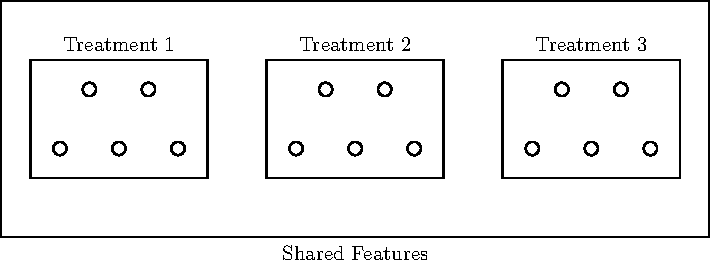
\includegraphics[width=0.7\linewidth]{chapters/conclusion/nestedDesign.pdf}
    \caption[A diagram of a controlled experiment with replications.]{A diagram of a controlled experiment with replications. Each circle represents a unique replicate with its own distinct features (parameters). The rectangular boxes represent different treatments, each containing shared features for their respective replications. The entire experiment is encased in a larger rectangle indicating features common across all treatments.}
    \label{fig:controlled_experiment}
\end{figure}

The theoretical analysis of the PIF algorithm presented in Chapter~\ref{chpt:mpif} can readily be extended to include this extra layer of parameter nesting, though existing software cannot immediately be used to handle this general scenario.

\subsection*{Parameter estimation using automatic differentiation}

Recent methodological work on automatic differentiation for particle filters has shown potential for speeding up inference for POMP models \citep{tan24}.
The MPIF algorithm presented in Chapter~\ref{chpt:mpif} can be immediately combined with this promising methodology in the panel setting, as the method of \citet{tan24} requires a warm restart in order to successfully converge to the MLE.

Additionally, the combination of MPIF and automatic differentiation may facilitate the use of shallow neural networks to be used in conjunction with mechanistic models.
As an example, consider a continuous time compartmental model outlined in Appendix~\ref{subsec:smcs}.
Transition rates between compartments are generally expressed as functions of latent and exogenous variables, denoted $f(\bm{X}(t), \bm{Z}(t))$.
Rather than predetermining the function $f$, automatic differentiation software may enable treating $f$ as a flexible function that needs to be estimated.
A similar idea has been explored previously \citep{noordijk24,dandekar20}, though only in the context of deterministic ODE models, or SDE models with non-mechanistic latent dynamics \citep{lin24}.
In the later approach, a neural network is used to approximate an unknown function that describes the latent process. 
This has the advantage of allowing flexible description of latent states, but it loses the benefits of being mechanistic.
Automatic differentiation for particle filters instead may allow for retaining the general mechanistic framework of a SSM, while permitting extra flexibility for model components where a mechanistic representation is not readily available \citep{dandekar20}. 

\subsection*{Applications in Ecology, Agriculture, and Epidemiology}

The MPIF algorithm presented in Chapter~\ref{chpt:mpif} results in an improved capacity to calibrate PanelPOMP models to data via maximum likelihood.
Given the prevalence of panel data and applications of POMP models to univariate time series, this innovation may lead to a number of collaborative research projects in epidemiology.
Iterated filtering has been a poplar approach for modeling infectious disease outbreaks at a single measurement location using nonlinear, overdispersed stochastic models \citep[e.g.,][]{stocks20}. 
The MPIF algorithm facilitates fitting similar models to outbreaks measured at various distinct locations, which can be particularly useful at the onset of disease outbreaks, when there is limited amounts of data available at a single measurement location.

In addition to novel applications in epidemiology, there are several areas of research where I feel that PanelPOMP methodology can lead to novel scientific insights.
Two application areas I feel are particularly promising are fisheries and agriculture.
Fisheries have a rich history of using state space models, though typically inference is performed using Lapacian approximations of the likelihood \citep[e.g.,][]{auger17}.
In addition to comparing whether this approach is a more reliable approximation that those built on sequential Monte Carlo methodologies, studying infectious diseases prevalent in native river and lake species may be uniquely well suited for PanelPOMP methodology: population dynamics in each river or lake are independent from other locations, yet share many similar features that should be estimated simultaneously.
Alternatively, the MPIF methodology may be used to model the nonlinear stochastic dynamics that arise from distinct fish populations competing for the same finite resources \citep{rosenthal22}.
Fish populations exhibit many of the same obstacles for inference that were outlined by \citet{bjornstad01}, and iterated filtering based algorithms have been successfully used to the same challenges in infectious disease outbreaks.

Livestock populations also exhibit nonlinear, stochastic features of biological systems, and may be well suited for applying PanelPOMP methodology.
Recently published research on livestock management \citep{skolstrup22} used linear Gaussian state space models to estimate the effects of interventions at dairy farms, and methodologies enabling nonlinear models may be a natural next step.
The MPIF algorithm may be used to fit nonlinear SSMs for large collections independent time series data, and could be useful for controlling infectious disease outbreaks such as recent avian flu outbreaks \citep{pinotti24}.

\subsection*{Likelihood based inference for ARIMA models}

In Chapter~\ref{chpt:arima}, a new algorithm was presented for performing maximum likelihood estimation for the parameters of an ARIMA model.
This project resulted in the development of an R package called \code{arima2}, which has already been downloaded more than the majority of R packages available on the Comprehensive R Archive Network (CRAN).
Given the importance of ARIMA models to modern science, additional efforts to improve both the algorithm and improve access to the algorithm are warranted.
For instance, a Python package that implements the algorithm should be built in order to provide access to help practitioners that prefer the Python language for data analysis.
Additional modifications to the algorithm may could include stratified sampling of parameter coefficients.
Alternatively, theoretical developments that provide bounds on the number of local optima could be explored. 


% Appendices
\appendix
% \input{appendices/arima2/pythonComparison}
\input{appendices/arima2/appendixArima2}
\chapter{Appendix for Chapter 3}
\label{chpt:appendix_haiti}


\section{Model Diagrams}\label{sec:appendix_haiti_diagrams}

Each of the dynamic models considered in this manuscript can be fully described using the model descriptions in the manuscript, coupled with the additional information described in Sections 2 and 3 of this supplement.
Despite this, diagrams of dynamic systems are often helpful to understand the equations.
In this section, we give three diagrams representing Models~1--3, respectively.
Because the models are defined by their mathematical equations and numeric implementation, these diagrams are not unique visual representations of the model.
Alternative representations that may be helpful in understanding the models explored in this paper are provided in the supplement material of \citet{lee20}.

\begin{figure}[!ht]
%%%%% SEAIR diagram
\begin{center}
  \resizebox{0.9\textwidth}{!}{
    \Large
    \setlength{\unitlength}{5pt}
    \begin{picture}(100,95)(0,15)
      \thicklines

      % Unvaccinated Compartments
      \put(10,63){\framebox(6,6){$\mathrm{S}_0$}}
      \put(34,63){\framebox(6,6){$\mathrm{E}_0$}}
      \put(58,71){\framebox(6,6){$\mathrm{A}_0$}}
      \put(82,63){\framebox(6,6){$\mathrm{R}_0$}}
      \put(58,55){\framebox(6,6){$\mathrm{I}_0$}}

      % Births
      \put(1, 66){\vector(1, 0){8}}
      \put(4, 68){$\muBirth$}

      % S_0 -> E_0
      \put(17,66){\vector(1,0){16}}
      \put(22,67){$\lambda(t)$}

      % E_0 -> A_0
      \put(41,67.5){\vector(2.1,1){16}}
      % \put(37, 72){$\muEI\big(1-\symptomFrac_{\vaccCounter}(t)\big)$}

      % E_0 -> I_0
      \put(41,65.5){\vector(2.1,-1){16}}

      % A_0 -> R_0
      \put(65,74){\vector(2.1,-1){16}}

      % I_0 -> R_0
      \put(65,59){\vector(2.4,1){16}}

      % R_0 -> S_0
      \cbezier(84,70)(75, 95)(23,95)(14,70)
      \put(14,70){\vector(-1, -2){0.3}}

      % Unvaccinated death rates
      \put(13, 70){\vector(0, 1){10}}
      \put(11, 74){$\muDeath$}

      \put(37, 70){\vector(0, 1){10}}
      \put(35, 74){$\muDeath$}

      \put(61, 78){\vector(0, 1){9}}
      \put(59, 80){$\muDeath$}

      \put(61, 62){\vector(1.5, 2){6}}
      \put(61.5, 65.5){$\muDeath$}

      \put(85, 70){\vector(0, 1){10}}
      \put(83, 74){$\muDeath$}

      % Vaccinated Compartments
      \put(10,37){\framebox(6,6){$\mathrm{S}_\vaccCounter$}}
      \put(34,37){\framebox(6,6){$\mathrm{E}_\vaccCounter$}}
      \put(58,45){\framebox(6,6){$\mathrm{A}_\vaccCounter$}}
      \put(82,37){\framebox(6,6){$\mathrm{R}_\vaccCounter$}}
      \put(58,29){\framebox(6,6){$\mathrm{I}_\vaccCounter$}}

      % S -> E
      \put(17,40){\vector(1,0){16}}
      \put(22,41){$\lambda(t)$}

      % E -> A
      \put(41,40.5){\vector(2.1,1){16}}

      % E -> I
      \put(41,39.5){\vector(2.1,-1){16}}

      % A -> R
      \put(65,48){\vector(2.1,-1){16}}

      % I -> R
      \put(65,32){\vector(2.1,1){16}}

      % R -> S
      \cbezier(84, 36)(75, 10)(23, 10)(14, 36)
      \put(14,36){\vector(-1, 2){0.3}}

      % Vaccinated death rates
      \put(13, 36){\vector(0, -1){10}}
      \put(11, 31){$\muDeath$}

      \put(37, 36){\vector(0, -1){10}}
      \put(35, 31){$\muDeath$}

      \put(61, 28.5){\vector(0, -1){9}}
      \put(59, 24){$\muDeath$}

      \put(61, 44){\vector(1.5, -2){6}}
      \put(62, 38){$\muDeath$}

      \put(85, 36){\vector(0, -1){10}}
      \put(83.2, 30.2){$\muDeath$}

      % S_0 -> S_\vaccCounter
      \multiput(13,62)(0,-2){9}{\line(0,-1){1}}
      \put(13, 43.5){\vector(0, -1){0}}

      % E_0 -> E_\vaccCounter
      \multiput(37,62)(0,-2){9}{\line(0,-1){1}}
      \put(37, 43.5){\vector(0, -1){0}}

      % R_0 -> R_\vaccCounter
      \multiput(85,62)(0,-2){9}{\line(0,-1){1}}
      \put(85, 43.5){\vector(0, -1){0}}

      % A_0 -> A_\vaccCounter
      \multiput(57.5,72)(-1.9, 0){3}{\line(-1, 0){0.9}}
      \put(52.2, 72){\line(-2.1, -1){1}}
      \multiput(51,71)(0, -2){11}{\line(0, -1){1}}
      \put(52.2, 49){\line(-2.1, 1){1}}
      \multiput(54,49)(1.9, 0){2}{\line(-1, 0){0.9}}
      \put(57, 49){\vector(1, 0){0}}

      % I_0 -> I_\vaccCounter
      \multiput(65, 57.5)(1.9, 0){3}{\line(1, 0){0.9}}
      \put(70.6, 57.5){\line(2.1, -1){1}}
      \multiput(72, 56.5)(0, -2){13}{\line(0, -1){1}}
      \put(72, 30.9){\line(-2, -1.2){0.9}}
      \multiput(65.6, 30.2)(1.9, 0){3}{\line(1, 0){0.9}}
      \put(64.5, 30.2){\vector(-1, 0){0}}

    \end{picture}
  }
\end{center}
\caption[Flow diagram of Haiti-cholera model (Model 1).]{Flow diagram of Haiti-cholera model (Model 1).}\label{fig:flow_diagram}
\end{figure}


\begin{figure}[!h]
%%%%% SEAIR diagram
\begin{center}
  \resizebox{\textwidth}{!}{
    \Large
    \setlength{\unitlength}{5pt}
    \begin{picture}(100,95)(0,15)
      \thicklines

      % Unvaccinated Compartments
      \put(10,63){\framebox(6,6){$\mathrm{S}_{u0}$}}
      \put(34,69){\framebox(6,6){$\mathrm{E}_{u0}$}}
      \put(58,77){\framebox(6,6){$\mathrm{A}_{u0}$}}
      \put(82,77){\framebox(6,6){$\mathrm{R^A}_{u0}$}}
      \put(82,61){\framebox(6,6){$\mathrm{R^I}_{u0}$}}
      \put(58,61){\framebox(6,6){$\mathrm{I}_{u0}$}}

      % % S_0 -> E_0
      \put(17,66){\vector(3,1.1){16}}

      % % E_0 -> A_0
      \put(41,72.5){\vector(2.1,1){16}}

      % % E_0 -> I_0
      \put(41,71.5){\vector(2.1,-1){16}}

      % % A_0 -> R_0
      \put(65,80.5){\vector(1,0){16}}

      % A_uz -> W_u
      \put(58,39){\framebox(6,6){$\mathrm{A}_{u\vaccCounter}$}}
      \qbezier[25](60.5, 46)(51, 52)(42, 53)
      \put(42, 53){\vector(-1, 0.1){0.5}}

      % A_uz -> W_u
      \qbezier[25](60.5, 60)(51, 54)(42, 54)
      \put(42, 54){\vector(-1, -0.1){0.5}}

      % I_uz -> W_u
      \qbezier[30](60.5,30)(48, 45)(40, 50)
      \put(40, 50){\vector(-1, 0.8){0.5}}

      % A_u0 -> W_u
      \qbezier[29](60.5,76)(48, 61)(40.6, 57)
      \put(40.8, 57.1){\vector(-1, -0.7){0.5}}

      % % I_0 -> R_0
      \put(65,63.5){\vector(1,0){16}}

      % % Vaccinated Compartments
      \put(10,37){\framebox(6,6){$\mathrm{S}_{u\vaccCounter}$}}
      \put(34,31){\framebox(6,6){$\mathrm{E}_{u\vaccCounter}$}}
      \put(58,39){\framebox(6,6){$\mathrm{A}_{u\vaccCounter}$}}
      \put(82,39){\framebox(6,6){$\mathrm{R^A}_{u\vaccCounter}$}}
      \put(58,23){\framebox(6,6){$\mathrm{I}_{u\vaccCounter}$}}
      \put(82,23){\framebox(6,6){$\mathrm{R^I}_{u\vaccCounter}$}}

      % R_0 -> S_0
      \cbezier(85,22)(80, 8)(18,8)(12,36)
      \put(12.1,35.5){\vector(-1, 3.5){0.3}}

      \cbezier(85,38)(80, 12)(18,15)(14,36)
      \put(14.1,35.5){\vector(-1, 3.5){0.3}}


      % R_0 -> S_0
      \cbezier(85,84)(80, 100)(18,100)(12,70)
      \put(12.1,70.5){\vector(-1, -3.5){0.3}}

      \cbezier(85,68)(80, 95)(18, 92)(14,70)
      \put(14.1,70.5){\vector(-1, -3.5){0.3}}

      % % S -> E
      \put(17,40){\vector(3,-1.1){16}}

      % % E -> A
      \put(41,34.5){\vector(2.1,1){16}}

      % % E -> I
      \put(41,33.5){\vector(2.1,-1){16}}

      % % A -> R
      \put(65,42.5){\vector(1,0){16}}

      % % I -> R
      \put(65,25.5){\vector(1,0){16}}

      % S_0 -> S_\vaccCounter
      \multiput(12,62)(0,-2){9}{\line(0,-1){1}}
      \put(12, 44){\vector(0, -1){0}}

      % S_0 -> S_\vaccCounter
      % Wanning vaccine efficacy
      \multiput(14,44)(0,2){9}{\line(0,1){1}}
      \put(14, 62){\vector(0, 1){0}}


      \put(37, 54){\circle{7}}
      \put(35, 53){$\mathrm{W_u}$}

      \qbezier[10](32.5, 54)(29.5, 54)(26.5, 54)
      \put(26, 54){\vector(-1, 0){0.1}}
      \put(28, 55){$\Wremoval$}

    \end{picture}
  }
\end{center}
\caption[Flow diagram of Haiti-cholera model (Model 2).]{Flow diagram of Haiti-cholera model (Model 2). This is a constant population model, there are no births/deaths. Vaccinations are assumed to only be given to susceptible individuals, and vaccine immunity wanes only with susceptible vaccinated individuals.}\label{fig:flow_diagram2}
\end{figure}


\begin{figure}[!h]
%%%%% SEAIR diagram
\begin{center}
  \resizebox{\textwidth}{!}{
    \Large
    \setlength{\unitlength}{5pt}
    \begin{picture}(100,85)(0,15)

    % COMPARTMENTS
    \put(39, 50){\circle{6}}
    \put(37, 49){$\mathrm{W}_{u}$}

    \put(8, 55){\framebox(6, 6){$\mathrm{S_{u0}}$}}
    \put(8, 39){\framebox(6, 6){$\mathrm{S_{u\vaccCounter}}$}}
    \put(36, 62.5){\framebox(6, 6){$\mathrm{A_{u}}$}}
    \put(36, 31.5){\framebox(6, 6){$\mathrm{I_{u}}$}}
    \put(56, 55){\framebox(6, 6){$\mathrm{R^1_{u0}}$}}
    \put(71, 55){\framebox(6, 6){$\mathrm{R^2_{u0}}$}}
    \put(86, 55){\framebox(6, 6){$\mathrm{R^3_{u0}}$}}
    \put(56, 39){\framebox(6, 6){$\mathrm{R^1_{u\vaccCounter}}$}}
    \put(71, 39){\framebox(6, 6){$\mathrm{R^2_{u\vaccCounter}}$}}
    \put(86, 39){\framebox(6, 6){$\mathrm{R^3_{u\vaccCounter}}$}}

    % INDIVIDUAL MOVEMENT
    % S_u0 -> A_u
    \put(15, 58.5){\vector(3, 1.2){20}}

    % S_u0 -> I_u
    \put(15, 57.5){\vector(1, -1.1){20}}

    % S_uz -> I_u
    \put(15, 41.5){\vector(3, -1.2){20}}

    % S_uz -> A_u
    \put(15, 42.5){\vector(1, 1.1){20}}

    % I_u -> R_u0
    \put(43, 66){\vector(2, -1){12}}

    % A_u -> R_uz
    \multiput(43, 64)(1.25, -1.6){12}{\line(1, -1.3){0.7}}
    \put(57, 46){\vector(1, -1.3){0.2}}

    \put(43, 36){\vector(1.7, 2){15}}

    \multiput(60, 54)(0, -2){4}{\line(0, -1){1}}
    \put(60, 46){\vector(0, -1){0.5}}

    \multiput(74, 54)(0, -2){4}{\line(0, -1){1}}
    \put(74, 46){\vector(0, -1){0.5}}

    \multiput(89, 54)(0, -2){4}{\line(0, -1){1}}
    \put(89, 46){\vector(0, -1){0.5}}

    \put(63, 58){\vector(1, 0){7}}
    \put(78, 58){\vector(1, 0){7}}

    \put(63, 42){\vector(1, 0){7}}
    \put(78, 42){\vector(1, 0){7}}

    \multiput(39, 61.5)(0, -1){8}{\line(0, -1){0.3}}
    \put(39,54){\vector(0, -1){0.5}}

    \multiput(39, 38.5)(0, 1){8}{\line(0, 1){0.3}}
    \put(39,46){\vector(0, 1){0.5}}

    \cbezier(89,62)(80, 85)(20, 85)(12,62)
    \put(12.2,62.5){\vector(-1, -3.5){0.3}}

    \cbezier(89,38)(80, 15)(20, 15)(12,38)
    \put(12.2,37.5){\vector(-1, 3.5){0.3}}

    \multiput(11, 54)(0, -2){4}{\line(0, -1){1}}
    \put(11, 46){\vector(0, -1){0.5}}

    % DEMOGRAPHY
    % -> S
    \put(0, 58){\vector(1, 0){7}}
    \put(1, 59){$\mathrm{\mu_{\demography S_{u0}}}$}

    % S Death
    \put(10, 62){\vector(0, 1){7}}
    \put(8, 64){$\mathrm{\muDeath}$}
    \put(10, 38){\vector(0, -1){7}}
    \put(8, 34){$\mathrm{\muDeath}$}

    % A + I death
    \put(39, 69.5){\vector(0, 1){7}}
    \put(37, 71.5){$\mathrm{\muDeath}$}

    \put(39, 31.5){\vector(0, -1){7}}
    \put(30, 27.5){$\mathrm{\muDeath + \choleraDeath}$}

    % R Death
    \put(59, 62){\vector(0, 1){7}}
    \put(57, 64){$\mathrm{\muDeath}$}

    \put(74, 62){\vector(0, 1){7}}
    \put(72, 64){$\mathrm{\muDeath}$}

    \put(59, 38){\vector(0, -1){7}}
    \put(57, 34){$\mathrm{\muDeath}$}

    \put(74, 38){\vector(0, -1){7}}
    \put(72, 34){$\mathrm{\muDeath}$}

    \put(93, 42){\vector(1, 0){7}}
    \put(95.5, 43){$\mathrm{\muDeath}$}

    \put(93, 58){\vector(1, 0){7}}
    \put(95.5, 59){$\mathrm{\muDeath}$}

    % W death
    \multiput(43, 50)(1, 0){7}{\line(1, 0){0.2}}
    \put(50.2, 50){\vector(1, 0){0.5}}
    \put(44, 51){$\mathrm{\Wremoval}$}

    \end{picture}
  }
\end{center}
\caption[Flow diagram of Haiti-cholera model (Model 3).]{Flow diagram of Haiti-cholera model (Model 3). This model assumes a constant population while also including a mechanism for births/deaths; all deaths are balanced by births into the unvaccinated susceptible compartment, so the birth rate $\mu_{\demography S_{u0}}$ corresponds to the sum total deaths from the remaining compartments. The model assumes that symptomatic individuals will not be vaccinated, hence no vaccination arrow exiting the $I_u0$ compartment.}\label{fig:flow_diagram3}
\end{figure}


\section{Markov chain and differential equation interpretations of compartment flow rates}\label{sec:appendix_haiti_details}

In the Materials and methods Section of the main article, we define compartment models in terms of their flow rates.
For a discrete population model, these rates define a Markov chain.
For a continuous and deterministic model, the rates define a system of ordinary differential equations.
Here, we add additional details to clarify the mapping from a collection of rate functions to a fully specified process.
Our treatment follows \cite{breto09}.

A general compartment model is a vector-valued process $X(t)=(X_1(t),\dots,X_c(t))$ denoting the (integer or real-valued) counts in each of $c$ compartments, where $t$ is any continuous value in the interval  $\left[t_0, \infty\right)$ for some real valued starting time $t_0$.
The compartments may also have names, but to set up general notation we simply refer to them by their numerical index.
The basic characteristic of a compartment model is that $X(t)$ can be written in terms of the flows $N_{ij}(t)$ from $i$ to $j$.
A flow into compartment $i$ from outside the system is denoted by $N_{\demography i}$, and a flow out of the system from compartment $i$ is denoted by $N_{i\demography}$.
We call $\demography$ a source/sink compartment, though it is an irregular compartment since $X_{\demography}(t)$ is not defined.
These flows are required to satisfy a ``conservation of mass'' identity:
\begin{equation}
X_i(t)=X_i(t_0)+N_{\demography i}(t) - N_{i\demography}(t) + \sum_{j\neq
i}N_{ji}(t)-\sum_{j\neq i}N_{ij}(t). \label{eq:conservation}
\end{equation}
Each {\emph flow} $N_{ij}(t)$ is associated with a {\emph rate} function
$\mu_{ij}=\mu_{ij}(t,X(t))$, where we include the possibility that $i$ or $j$ takes value $\demography$.

There are different ways to use a collection of rate functions to build a fully specified model.
We proceed to describe the ones we use in this paper: via a system of ordinary differential equations (Sec.~\ref{subsec:ode}), a simple Markov counting system (Sec.~\ref{subsec:smcs}), and an over-dispersed Markov counting system (Sec.~\ref{subsec:odmcs}). Other representations include stochastic differential equations driven by Gaussian noise or Gamma noise \cite{bhadra11}.

\subsection{Ordinary differential equation (ODE) interpretation}
\label{subsec:ode}

A basic deterministic specification is
\begin{equation}
\label{eq:ode1}
dN_{ij}/dt = \mu_{ij}\big(t,X(t) \big) X_i(t), \hspace{3mm} i\in \seq{1}{c}, \hspace{3mm} j\in \seq{1}{c} \cup\{\demography\}, \hspace{3mm} i\neq j,
\end{equation}
where $\mu_{ij}\big(t,X(t)\big)$ is called a per-capita rate or a unit rate.
Flows into the system require special treatment since $X_i(t)$ in \myeqref{eq:ode1} is not defined for $i=\demography$.
Instead, we specify
\begin{equation}
\label{eq:ode2}
dN_{\demography i}/dt = \mu_{\demography i}\big(t,X(t) \big).
\end{equation}
This is the the interpretation and implementation used for Model~2 in our study.

\subsection{Simple Markov counting system interpretation}
\label{subsec:smcs}
A continuous time Markov chain can be specified via its infinitesimal transition probabilities.
A basic approach to this is to define
\begin{eqnarray}
\label{eq:smcs1}
\prob\big[ N_{ij}(t+\delta)-N_{ij}(t)=0 \given X(t)\big]
 &=& 1-\delta \mu_{ij}\big(t,X(t)\big)X_i(t) + o(\delta),
\\
\label{eq:smcs2}
\prob\big[ N_{ij}(t+\delta)-N_{ij}(t)=1 \given X(t)\big]
 &=& \delta \mu_{ij}\big(t,X(t)\big)X_i(t) + o(\delta),
\end{eqnarray}
for $i\in \seq{1}{c}$ and $j\in\seq{1}{c}\cup\{\demography\}$ with $i\neq j$.
As with the ODE case, we need special attention for flows into the system, and we define
\begin{eqnarray}
\label{eq:smcs3}
\prob\big[ N_{\demography i}(t+\delta)-N_{\demography i}(t)=0 \given X(t)\big]
 &=& 1-\delta \mu_{\demography i}\big(t,X(t)\big) + o(\delta),
\\
\label{eq:smcs4}
\prob\big[ N_{\demography i}(t+\delta)-N_{\demography i}(t)=1 \given X(t)\big]
 &=& \delta \mu_{\demography i}\big(t,X(t)\big) + o(\delta).
\end{eqnarray}
Together with the initial conditions $X(0)$, equations \myeqref{eq:smcs1}--\myeqref{eq:smcs4} define a Markov chain.
Each flow is a simple counting process, meaning a non-decreasing integer-valued process that only has jumps of size one.
We therefore call the Markov chain a simple Markov counting system (SMCS).
The infinitesimal mean of every flow is equal to its infinitesimal variance \cite{breto11} and so an SMCS is called equidispersed.
We note that the special case of Model~1 used by \cite{lee20} (with $\sigmaProc = 0$) is an SMCS.
To permit more general mean-variance relationships for a Markov counting system, we must permit jumps of size greater than one.
The utility of over-dispersed models, where the infinitesimal variance of the flow exceeds the infinitesimal mean, has become widely recognized \cite{stocks20,he10}.

\subsection{Overdispersed Markov counting system interpretation}
\label{subsec:odmcs}

Including white noise in the rate function enables the possibility of an over-dispersed Markov counting system \cite{breto11,breto09,he10}.
Since rates should be non-negative, Gaussian noise is not appropriate and gamma noise is a convenient option that has found various applications \cite{romero-severson15, subramanian20}.
Specifically, we consider a model given by
\begin{equation}
\label{eq:odmcs1}
\mu_{ij}\big(t,X(t)\big) = \bar\mu_{ij}\big(t,X(t)\big) \, d\Gamma_{ij}(t)/dt,
\end{equation}
where $\Gamma_{ij}(t)$ is a stochastic process having independent gamma distributed increments, with
\begin{equation}
\label{eq:odmcs2}
\E\big[\Gamma_{ij}(t)\big] = t, \quad \var\big[\Gamma_{ij}(t)\big] = \sigma_{ij}^2 t.
\end{equation}
Formally interpreting the meaning of \myeqref{eq:odmcs1} is not trivial, and we do so by constructing a Markov process $X(t)$ as the limit of the Euler scheme described in Section~\ref{sec:numerics}, below.
Therefore, the numerical scheme in Sec.~\ref{sec:numerics} can be taken as a definition of the meaning of \myeqref{eq:odmcs1}.
The Markov chain defined by the limit of this Euler scheme as the step size decreases is an over-dispersed Markov counting system, with the possibility of instantaneous jumps of size greater than one \cite{breto11}.

\section{Numerical solutions to compartment models}
\label{sec:numerics}

Models may be fitted and their implications assessed via numerical solutions (i.e., simulations) from the model equations.
All the analyses we consider have this simulation-based property, known as plug-and-play or equation-free or likelihood-free.
The numerical solutions to the model are arguably of more direct scientific interest than the exact solutions to the postulated equations.
For ODE models, numerical methods are well studied and a standard numerical solution package such as \code{deSolve} in \code{R} is adequate for many purposes.
For SMCS and ODMCS models, exact schemes are feasible when the number of events is small, which may be the case for small populations.
However, for applicability to larger populations, we use instead the following Euler scheme.
Write $\delta$ for an Euler time step, and $\Delta N_{ij}$ for the numerical approximation to $N_{ij}(t+\delta)-N_{ij}(t)$ given $X(t)$.
For each $i$ and $j$ in $\seq{1}{c} \cup \{\demography\}$ with $i \neq j$, we draw independent Gamma distributed noise increments with mean $\delta$ and variance $\sigma_{ij}^2 \delta$, denoted using a mean-variance parameterization of the gamma distribution as
\begin{equation}
\label{eq:numerics1}
\Delta\Gamma_{ij} \sim \mathrm{gamma}(\delta, \sigma_{ij}^2 \delta).
\end{equation}
In the case of an SMCS model, $\sigma_{ij}=0$ for all $i$ and $j$, so we have $\Delta\Gamma_{ij}=\delta$.
Then, for $i\neq \demography$ and $j\neq i$, and writing
\begin{equation}
\label{eq:numerics2}
\mu_{ij}=\bar\mu_{ij}\big(t,X(t)\big) \Delta\Gamma_{ij} / \delta,
\end{equation}
we calculate transition probabilities
\begin{eqnarray}
\label{eq:numerics3}
p_{ij} &=& \exp\left\{-\sum_{k\in 1:c \, \cup \{\demography\}} \mu_{ik} \, \delta \right\}
\frac{\mu_{ij}}{\sum_{k\in 1:c\cup \{\demography\}} \mu_{ik}},
\\
\label{eq:numerics4}
p_{ii} &=& 1 - \sum_{j\neq i} p_{ij}.
\end{eqnarray}
These probabilities correspond to competing hazards for every individual in compartment $i$ to transition to some compartment $j$, interpreting $j=i$ to mean that the individual remains in $i$.
Then, $\big(\Delta N_{i1},\dots,\Delta N_{ic},\Delta N_{i\demography}\big)$ has the multinomial distribution where $X_i(t)$ individuals are allocated independently to $\seq{1}{c}\cup\{\demography\}$ with probabilities given by \eqref{eq:numerics3} and \eqref{eq:numerics4}.
We use the \code{reulermultinom} function in the \code{pomp} package to draw from this multinomial distribution.

Different treatments of demographic flows---such as birth, death, immigration and emigration---are possible.
For the case $i=\demography$, the treatment used by Model~1 is to set
\begin{equation}
\label{eq:numerics6}
\Delta N_{\demography j} \sim \mathrm{poisson}( \mu_{\demography j} \delta),
\end{equation}
an independent Poisson random variable with mean $\mu_{\demography j} \delta$.

Models~2 and 3 used an alternative approach, balancing the total number of flows in and out of the compartment, i.e., $\sum_{i}N_{\demography i}(t) = \sum_{i}N_{i \demography}(t)$, in order to make the model consistent with the known total population.
In this case, we formally model the death rate as a rate of returning to the susceptible class $S$, and use external transitions from $\demography$ into $S$ to describe only net population increase.




%%%%%%%%%% START

\section{Confidence Intervals for Model Parameters}\label{sec:appendix_haiti_ci}

In this section we provide confidence intervals for all model parameters, excluding those that take unique values for each spatial unit.
For each model and parameter, we use principles of profile likelihood to obtain confidence intervals \citep{pawitan01}.
Due to the non-linear and stochastic nature of Models~1 and 3, exact evaluations of the profile log-likelihood are difficult to obtain.
Instead, the log-likelihood at each point of the profile is estimated using via Monte-Carlo based particle filter methods.
We therefore obtain confidence intervals for the parameters of Model~1 and Model~3 using the Monte Carlo adjust profile (MCAP) algorithm \citep{ionides17}.

Profile confidence intervals for nonlinear POMP models are require a large number of computations. In the Model~1 and Model~3 subsections, we mention the total computational expense of each profile log-likelihood evaluation. Each subsection also provide figures that show the curvature of the profile log-likelihood near the MLE (Figures~\ref{fig:m1Profs}--\ref{fig:m3Profs}).
In these figures, the parameter values are shown on the transformed scale in which the profile was calculated.

\subsection{Model~1 parameters}

Parameter estimates for Model~1, along with the MCAP confidence intervals for the estimate, are given in Table~\ref{tab:mod1CI}.
Figure~\ref{fig:m1Profs} displays the Monte Carlo evaluations of the profile likelihood values, obtained using a particle filter.
The total computational burden of this profile likelihood search was 3631 hours, which was computed in parallel using 9675 separate jobs via the \texttt{batchtools} R package \cite{batchtools}.





\begin{figure}[ht]
\begin{knitrout}
\definecolor{shadecolor}{rgb}{0.969, 0.969, 0.969}\color{fgcolor}

{\centering \includegraphics[width=\maxwidth]{figure/m1Profs-1} 

}


\end{knitrout}
\caption[MCAP confidence intervals for Model 1 parameters.]{\label{fig:m1Profs}MCAP confidence intervals for Model 1 parameters. The vertical blue line indicates the smoothed MLE.}
\end{figure}

\begin{table}[!h]
\centering
\caption[Model~1 parameter estimates and confidence intervals.]{\label{tab:mod1CI}Model~1 parameter estimates and their corresponding confidence intervals, obtained via the MCAP algorithm.}
\vspace{2mm}
\begin{tabular}{|L{3.60cm}|C{2.1cm}|C{1.9cm}|C{3.95cm}|}
\hline
\centering \textbf{Mechanism} & \textbf{Parameter} & \textbf{MLE} & $\bm{95\%}$ \textbf{Confidence Interval} \\
\hline
\hline

 Seasonality & $\transmissionTrend$ & $-0.036$
   &
  $(-0.070, -0.008)$
\\
\hline

 Seasonality & $\transmission_1$ & $1.417$
   &
  $(1.277, 1.811)$
\\
\hline

 Seasonality & $\transmission_2$ & $1.169$
   &
  $(0.937, 1.445)$
\\
\hline

 Seasonality & $\transmission_3$ & $1.136$
   &
  $(0.990, 1.630)$
\\
\hline

 Seasonality & $\transmission_4$ & $1.140$
   &
  $(0.922, 1.389)$
\\
\hline

 Seasonality & $\transmission_5$ & $1.401$
   &
  $(1.261, 1.687)$
\\
\hline

 Seasonality & $\transmission_6$ & $0.988$
   &
  $(0.699, 1.132)$
\\
\hline

 Observation Variance & $\obsOverdispersion: \mathrm{Epi}$ & $279.147$
   &
  $(177.226, 990.191)$
\\
\hline

 Observation Variance & $\obsOverdispersion: \mathrm{End}$ & $78.326$
   &
  $(57.171, 204.654)$
\\
\hline

  Reporting Rate & $\reportRate$ & $0.679$
   &
  $(0.315, 0.761)$
\\
\hline

  Mixing Exponent & $\mixExponent$ & $0.978$
   &
  $(0.938, 0.999)$
\\
\hline

  Process noise {\footnotesize (wk\textsuperscript{1/2})} & $\sigmaProc: \mathrm{Epi}$ & $0.092$
   &
  $(0.085, 0.113)$
\\
\hline

  Process noise {\footnotesize (wk\textsuperscript{1/2})} & $\sigmaProc: \mathrm{End}$ & $0.118$
   &
  $(0.092, 0.179)$
\\
\hline

  Initial Values & $I_{0}(0)$ & $7298$
   &
  $(2572, \ensuremath{1.4415\times 10^{4}})$
\\
\hline

  Initial Values & $E_{0}(0)$ & $350$
   &
  $(1, \ensuremath{1.3671\times 10^{4}})$
\\
\hline

\end{tabular}
\end{table}

\subsection{Model~2 parameters}

Parameter estimates for Model~2, along with the profile likelihood confidence intervals for each estimate, are given in Table~\ref{tab:mod2CI}.
Figure~\ref{fig:m2Profs} displays the profile log-likelihood curve near the MLE.
In Table~\ref{tab:mod2CI}, the confidence interval for $\muRS^{-1}$, the duration of natural immunity due to cholera infection, is arbitrarily large (going to infinity).
This is possible because the parameter that was estimated was $\muRS$, and the true MLE for this parameter is zero (see Figure~\ref{fig:m2Profs}).
This suggests that the fitted model favors a regime where reinfection events are not possible.
Similarly, the MLE for the parameter $\transmission$, which controls the amount of cholera transmission from human to human, is zero.
Because Model~2 fails to describe the incidence data as well as a simple statistical benchmark, we must be careful to not interpret these results as evidence that reinfections and human-to-human infection events do not occur.
Instead, we may consider this as additional evidence of model mispecification.



\begin{figure}[ht]
\begin{knitrout}
\definecolor{shadecolor}{rgb}{0.969, 0.969, 0.969}\color{fgcolor}

{\centering \includegraphics[width=\maxwidth]{figure/m2Profs-1} 

}


\end{knitrout}
\caption[MCAP confidence intervals for Model 2 parameters.]{\label{fig:m2Profs}MCAP confidence intervals for Model 2 parameters. The vertical blue line indicates the MLE.}
\end{figure}

\begin{table}[!h]
\centering
\caption[Model~2 parameter estimates and confidence intervals.]{\label{tab:mod2CI}Model~2 parameter estimates and their corresponding confidence intervals, obtained via profile likelihood.}
\vspace{2mm}
\begin{tabular}{|L{3.25cm}|C{2.1cm}|C{1.9cm}|C{4.2cm}|}
\hline
\centering \textbf{Mechanism} & \textbf{Parameter} & \textbf{MLE} & $\bm{95\%}$ \textbf{Confidence Interval} \\
\hline
\hline

 Human to water shedding {\small (wk\textsuperscript{-1})} & $\Wshed$ & $179.2$
   &
  $(144.6, 229.4)$
\\
\hline

 Water to Human Infection {\small (yr\textsuperscript{-1})} & $\beta_W$ & $1.098$
   &
  $(1.067, 1.128)$
\\
\hline

 Observation Variance & $\obsOverdispersion$ & $1.319$
   &
  $(1.291, 1.347)$
\\
\hline

 Seasonality & $\phaseParm$ & $0.974$
   &
  $(7.127, 7.381)$
\\
\hline

Human to Human Infection {\small (yr\textsuperscript{-1})} & $\transmission$ & $\ensuremath{5.97\times 10^{-15}}$\textsuperscript{*}
   &
  $[0, \ensuremath{2.3\times 10^{-6}})$
\\
\hline

Immunity {\small (yr)} & $\muRS^{-1}$ & $\ensuremath{1.4\times 10^{11}}$\textsuperscript{*}
   &
  $(1410, \inf)$
\\
\hline

\end{tabular}
\begin{flushleft}
\textsuperscript{*}As evident in Figure~\ref{fig:m2Profs}, the true MLE for these parameters is $0$ and $\infty$, respectively; this value could not be obtained numerically due to the parameter transformation applied to the parameter for the model fitting processes.
\end{flushleft}
\end{table}

\subsection{Model~3 parameters}

Parameter estimates for Model~3, along with the MCAP confidence intervals for the estimate, are given in Table~\ref{tab:mod3CI}.
Figure~\ref{fig:m3Profs} displays the Monte Carlo evaluations of the profile likelihood values, obtained using a particle filter.
The total computational burden of this profile likelihood search was 28938 hours, which was computed in parallel using 7568 separate jobs via the \texttt{batchtools} R package \cite{batchtools}.





\begin{figure}[ht]
\begin{knitrout}
\definecolor{shadecolor}{rgb}{0.969, 0.969, 0.969}\color{fgcolor}

{\centering \includegraphics[width=\maxwidth]{figure/m3Profs-1} 

}


\end{knitrout}
\caption[MCAP confidence intervals for Model 3 parameters.]{\label{fig:m3Profs}MCAP confidence intervals for Model 3 parameters. The vertical blue line indicates the smoothed MLE.}
\end{figure}

\begin{table}[!h]
\centering
\caption[Model~3 parameter estimates and confidence intervals.]{\label{tab:mod3CI}Model~3 parameter estimates and their corresponding confidence intervals, obtained via the MCAP algorithm.}
\vspace{2mm}
\begin{tabular}{|L{3.60cm}|C{2.1cm}|C{1.9cm}|C{4.3cm}|}
\hline
\centering \textbf{Mechanism} & \textbf{Parameter} & \textbf{MLE} & $\bm{95\%}$ \textbf{Confidence Interval} \\
\hline
\hline

 Process Noise {\footnotesize (wk\textsuperscript{1/2})} & $\sigmaProc$ & $0.218$
   &
  $(0.203, 0.230)$
\\
\hline

 Water Survival {\footnotesize (wk)} & $\Wremoval^{-1}$ & $0.108$
   &
  $(0.087, 0.110)$
\\
\hline

 Human to Water Shedding {\footnotesize $\frac{\mathrm{km^2}}{\mathrm{wk}}$} & $\Wshed$ & $\ensuremath{9.77\times 10^{-7}}$
   &
  $(\ensuremath{8.64\times 10^{-7}}, \ensuremath{1.25\times 10^{-6}})$
\\
\hline

 Asymptomatic Shedding & $\asymptomRelativeShed$ & $0.008$
   &
  $(0.0, 0.095)$
\\
\hline

 Seasonality & $\seasAmplitude$ & $1.000$
   &
  $(0.637, 1.432)$
\\
\hline

 Seasonality & $\rainfallExponent$ & $0.780$
   &
  $(0.498, 1.041)$
\\
\hline

 Reporting Rate & $\reportRate$ & $0.983$
   &
  $(0.789, 1.000)$
\\
\hline

 Observation Variance & $\obsOverdispersion$ & $88.578$
   &
  $(66.034, 132.563)$
\\
\hline

\end{tabular}
\end{table}

\section{Replication of Lee et al.~(2020) results}\label{sec:appendix_haiti_lee20}

In this article we claimed that we were able to obtain better fits to the observed data using the same models that were proposed by \citet{lee20}.
Along with visual comparisons to the data, this claim was supported by comparing likelihoods and AIC values in Table~2 in the manuscript.
Because model likelihoods were not provided by \citet{lee20}, it is necessary to replicate these models in order to obtain likelihood estimates.
Here we would like to thank the authors of \citet{lee20}, who provided detailed descriptions of their models, which enabled us to build on their work.
In the following subsections, we use our \code{R} package \code{haitipkg} to reproduce some of the results of \citet{lee20}.
This reproduction allows us to estimate the likelihoods of the \citet{lee20} version of Models~1--3, and also provides a demonstration of the importance and usefulness of reproducible research.

\subsection{Model~1 Replication}

The model was implemented by a team at Johns Hopkins Bloomberg School of Public Health (hereafter referred to as the Model~1 authors) in the \code{R} programming language using the \code{pomp} package \citep{king16}.
Original source code is publicly available with DOI: 10.5281/zenodo.3360991.
The final results reported by the Model~1 authors were obtained by using several different parameter sets rather than a single point estimate.
According to the supplement materials, this was because model realizations from a single parameter set retained substantial variability, but multiple realizations from a collection of parameter sets resulted in a reasonable visual fit to the data.
We are also inclined to believe that the use of multiple parameter values was in part intended to account for parameter uncertainty---the importance of which was discussed in the main text---an effort by the Model~1 authors that we applaud.
Simulations from each of the parameter sets, however, were treated with equal importance when being used to diagnose the model fit and make inference on the system.
This is problematic given Figures S8 and S9 of the supplement material, which suggest that some parameter sets that were used for inference may have been several hundred units of log-likelihood lower than other parameter sets that were simultaneously used to make forecasts.
Such a large difference in log-likelihoods is well beyond the threshold of statistical uncertainty determined by Wilks' theorem, resulting in the equal use of statistically inferior parameter sets in order to make forecasts and conduct inference on the system.

To fully reproduce the results of the Model~1 authors, it is necessary to use the exact same set of model parameters that were originally used to obtain the results presented by \citet{lee20}.
Because these parameter sets were not made publicly available, we relied on the source code provided by the Model~1 authors to approximately recreate the parameter set.
Due to software updates since the publication of the source code, we were unable to produce the exact same set of parameters.
Running the publicly available source code, however, resulted in a set of parameters that are visually similar to those used by the Model~1 authors (See Figures~\ref{fig:PlotEpiDist} and \ref{fig:plotEndParams}).
Furthermore, simulations using the set of parameters produced by the source code appear practically equivalent to those displayed by \citet{lee20} (See Figure~\ref{fig:plotMod1Sims}).



\begin{figure}[!h]
\begin{knitrout}
\definecolor{shadecolor}{rgb}{0.969, 0.969, 0.969}\color{fgcolor}

{\centering \includegraphics[width=\maxwidth]{figure/PlotEpiDist-1} 

}


\end{knitrout}
\caption[Replicating Model 1 epidemic phase parameter distributions]{\label{fig:PlotEpiDist}
Bivariate distributions of parameter estimates after fitting epidemic phase of the Model~1 following the procedure described by \citet{lee20}. Compare to Figure S8 in the supplement of \citet{lee20}.
}
\end{figure}





\begin{figure}[!h]
\begin{knitrout}
\definecolor{shadecolor}{rgb}{0.969, 0.969, 0.969}\color{fgcolor}

{\centering \includegraphics[width=\maxwidth]{figure/plotEndParams-1} 

}


\end{knitrout}
\caption[Replicating Model 1 endemic phase parameter distributions]{\label{fig:plotEndParams}
Bivariate distributions of parameter estimates after fitting endemic phase of the Model~1 following the procedure described by \citet{lee20}. Compare to Figure~S9 in the supplement of \citet{lee20}.
}
\end{figure}



\begin{figure}[!h]
\begin{knitrout}
\definecolor{shadecolor}{rgb}{0.969, 0.969, 0.969}\color{fgcolor}
\includegraphics[width=\maxwidth]{figure/plotMod1Sims-1} 
\end{knitrout}
\caption[Simulations from replicated Model 1]{\label{fig:plotMod1Sims}
Simulations from Model~1 using parameter sets that were generated by running source code provided by \citet{lee20}. Compare to Figure~S7 in the supplement of \citet{lee20}. The upper bound for the likelihood of this model is -3031.
}
\end{figure}

Because the model forecasts provided by \citet{lee20} come from various sets of parameters---which each correspond to a unique log-likelihood value---it is not obvious how one would obtain an estimate for the log-likelihood of the model that was used for simulations by the Model~1 authors.
One approach could be to calculate the logarithm of the weighted mean of the likelihoods for each parameter sets used to obtain the forecasts, where the weights are proportional to the number of times the parameter set was used.
However, in an effort to not underestimate the likelihood of the model of the Model~1 authors, we report the estimated log-likelihood as the log-likelihood value corresponding to the parameter set with the largest likelihood value, even though the majority of simulations were obtained using parameter sets with lower likelihood values.
In this sense, we consider the log-likelihood reported in Table~1 of the main text to be an upper-bound of the log-likelihood of the model used by \citet{lee20}.
For each parameter set, the log-likelihood was estimated using a particle filter, implemented as the \texttt{pfilter} function in the \texttt{pomp} package.

\subsection{Model~2 Replication}\label{sec:mod2rep}

Model~2 was developed by a team that consisted of members from the Fred Hutchinson Cancer Research Center and the University of Florida (hereafter referred to as the Model~2 authors).
While Model~2 is the only deterministic model we considered in our analysis, it contains perhaps the most complex descriptions of cholera in Haiti: Model~2 accounts for movement between spatial units; human-to-human and environment-to-human cholera infections; and transfer of water between spatial units based on elevation charts and river flows.

The source code that the Model~2 authors used to generate their results was written in the \code{Python} programming language, and is publicly available at \url{10.5281/zenodo.3360857} and its accompanying GitHub repository \url{https://github.com/lulelita/HaitiCholeraMultiModelingProject}.
In order to perform our analysis in a unified framework, we re-implemented this model in the \code{R} programming language using the \code{spatPomp} package \citep{asfaw24}, which facilitates the creation of meta-population models.
We note that the travel and water matrices used to implement the complex dynamics in Model~2 are not available in either the Zenodo archive or the GitHub repository;
instead, we obtained these matrices via personal correspondence with the Model~2 authors.
Using these matrices, and the point estimates for model parameters provided by \citet{lee20}, we created trajectories of the cholera dynamics and compared this to available data.
These trajectories, shown in Figure~\ref{fig:mod2rep}, are very similar to the trajectories shown in Figure~S15 of the supplement of \citet{lee20}.




\begin{figure}[!h]
\begin{knitrout}
\definecolor{shadecolor}{rgb}{0.969, 0.969, 0.969}\color{fgcolor}
\includegraphics[width=\maxwidth]{figure/plotModel2Rep-1} 
\end{knitrout}
\caption[Model~2 trajectories.]{\label{fig:mod2rep}
Model 2 trajectories using the \code{haitipkg}. Compare to Figure S15 in the supplement of \citet{lee20}.
}
\end{figure}

There are minor differences between Figure~\ref{fig:mod2rep} and Figure~S15 of \citet{lee20}.
While the discrepancy appears minor, the deterministic nature of Model~2 implies that an exact replication of model trajectories should be possible.
In this case, these discrepancies may possibly be attributed to implementing the model and plotting the model trajectory in two different programming languages.
Another potential explanation for the discrepancy is that the parameters that we used are only approximately the same as those used by \citet{lee20}.
For example, the parameters $\transmission$, $\Wbeta{}$ had reported values of $9.9 \times 10^{-7}$ and $4.03 \times 10^{-2}$, respectively (Table~S13 of the supplement material of \citet{lee20}), but were actually fit to data and therefore likely these values have been rounded.
Additionally, our implementation of Model~2 used a time scale of years and many of the parameters were reported on a weekly scale, so small differences may result due to unit conversions.
The collective effect of these small differences in model parameters likely will result in small differences in model trajectories.

Some additional concerns about being able to accurately replicate the results of \citet{lee20} are valid.
Details about the measurement models and how latent states were initialized for the epidemic model were not provided by \citet{lee20} and therefore these details must be inferred by looking at the provided source code.
According to repository comments, the files \code{fit\allowbreak In\allowbreak Pieces\allowbreak 3params\allowbreak Clean\allowbreak May2019\allowbreak Public.py} and \code{fit\allowbreak In\allowbreak Pieces\allowbreak Mu\allowbreak With\allowbreak Frac\allowbreak Sus\allowbreak Fixed\allowbreak All\allowbreak Infections\allowbreak Public.py} were used to fit the epidemic and endemic phases of the model respectively, although it is apparent that these exact files were not used to obtain the reported results since the files contain some variable-naming errors that make it impossible to run the files without making modifications \footnote{One example of why the code cannot be run that the file loads functions from a non-extant file named \code{choleraEqs.py} in line 13 rather than \code{cholera\allowbreak Eqs\allowbreak Public.py}.}.
The inability to replicate the results by \citet{lee20} by running the provided source code makes checking whether or not a our numeric implementation faithfully represents their results very difficult.
Additionally, the script that was said to been used to obtain the results reported by \citet{lee20} appears to use a different measurement model than what was described in the supplemental material, again making it difficult to fully replicate the result of \citet{lee20} without being able to easily run the provided source code.
In this case, we chose to use measurement model that considers only symptomatic individuals for both phases of the epidemic, as this seemed to visually match the results of \citet{lee20} most closely.

\subsection{Model~3 Replication}

Model~3 was developed by a team of researchers at the Laboratory of the Swiss Federal Institute of Technology in Lausanne, hereafter referred to as the Model~3 authors.
The code that was originally used to implement Model~3 is archived with the DOI: \url{10.5281/zenodo.3360723}, and also available in the public GitHub repository: \code{jcblemai/haiti-mass-ocv-campaign}.
Because the code was made publicly available, and final model parameters were reported in the supplementary material of \citet{lee20}, we were able to reproduce Model~3 by directly using the source code.
In Figure~\ref{fig:mod3rep}, we plot simulations from this model.
This figure can be compared to Figure S18 of \citet{lee20}.
We note that slight differences may be accounted for due to variance in the model simulations and the difference in programming language used to produce the figure.
Overall, the high standard of reproducibility that was achieved by the Model~3 authors facilitated the ability to readily replicate their model and results.



\begin{figure}[!h]
\begin{knitrout}
\definecolor{shadecolor}{rgb}{0.969, 0.969, 0.969}\color{fgcolor}
\includegraphics[width=\maxwidth]{figure/PlotMod3Rep-1} 
\end{knitrout}
\caption[Simulations from replicated Model 3]{\label{fig:mod3rep}
Simulations from Model~3.
Compare to Figure S18 in the supplement of \citet{lee20}.
}
\end{figure}



\section{Calibrating Model~3 to observed cases}\label{sec:appendix_haiti_mod3Cal}












In this section, we provide more detail on the process that was used to estimate the coefficients of Model~3.
In particular, we discuss why we decided to include additional model parameters---those that are associated with the behavior of the system during Hurricane Matthew---that were not considered by \cite{lee20}.
To calibrate this model, we used the iterated block particle filter (IBPF) method of \cite{ionides24}.
Due to the novelty of this algorithm, there exists only a few examples where the IBPF algorithm is used for data analysis \cite{li23,ionides24}, which is one motivation of the inclusion additional details related to fitting and diagnosing the model fit provided here.

Lee et al. (2020)~\cite{lee20} only estimated model parameters to a simplified version of Model~3 on a subset of the available data, as no method existed at the time of their publication to fit a fully coupled meta-population model to disease incidence data.
Building on their results, we fit the fully coupled version of Model~3 to (nearly) all available data, reserving only a few observations to use to calibrate the initial conditions of the model (see the supplement for initialization models for more details).
To maximize model likelihoods, we relied on parameter estimates obtained while calculating profile-likelihood confidence intervals, as this calculation requires many replicated IBPF searches.
In our preliminary investigations that were done prior to conducting a profile likelihood search, we found that it was necessary to use multiple searches for the MLE, periodically pruning away less successful searches.
To do this, the first collection of searches is performed by obtaining initial values for the parameters by uniformly sampling values from a predefined hypercube.
A subsequent refinement search used parameter values corresponding to the largest model likelihoods as starting parameter values.
The need for multiple searches does not appear to be uncommon, as a similar approach was used in \cite{ionides24}.
While computationally intensive, profile likelihoods proved to be an effective alternative to maximizing model likelihoods without the need to apply this multistage heuristic.

We use the iterative fitting / pruning technique described above to fit the fully coupled version of Model~3 proposed in \cite{lee20}.
The maximum likelihood we obtained after two rounds of searching was $\ensuremath{-1.7549\times 10^{4}}$, which is higher than the benchmark model ($\ensuremath{-1.7933\times 10^{4}}$).
While beating a simple associative benchmark is promising, this does not immediately imply that the model is a good description of the system.
Additional investigation of parameters estimates and their corresponding implications on model based conclusions should always be conducted.
For meta-population models, it is worth considering how well the model fits the data to each spatial unit.
% This can be done by looking at conditional log-likelihoods, which is part of the output of the \texttt{bpfilter} algorithm in the \texttt{spatPomp} package.
The likelihoods for each department, compared to the corresponding benchmark model, are displayed in Figure~\ref{fig:h3UnitLikes}.
The figure demonstrates that while the log-likelihood of the fitted model outperforms the auto-regressive negative binomial benchmark model at the aggregate level, Model~3 has lower likelihoods for some departments.

\begin{figure}[!ht]
\begin{knitrout}
\definecolor{shadecolor}{rgb}{0.969, 0.969, 0.969}\color{fgcolor}

{\centering \includegraphics[width=\maxwidth]{figure/h3UnitLikes-1} 

}


\end{knitrout}
\caption[Model~3 unit log-likelihoods.]{\label{fig:h3UnitLikes}Log-likelihoods of Model~3 for each department compared to the corresponding benchmark model prior to the inclusion of parameters that account for Hurricane Matthew.}
\end{figure}

In addition to considering the conditional log-likelihoods of each unit, one can consider conditional log-likelihoods of each observation.
When compared to a benchmark, this level of detail can provide useful information about which observations are well described by the model and which are not.
In Figure~\ref{fig:condLL}, we plot the conditional log-likelihoods of Model~3 for each observation.
Typically it is most useful to compare the conditional log-likelihoods of the model under consideration to a benchmark, as plotting only conditional log-likelihoods without a comparison may not be helpful.
In this case, however, the same insight can be drawn using a figure without a benchmark comparison, so we do not include the benchmark in order to avoid the issue of over-plotting.

\begin{figure}[!ht]
\begin{knitrout}
\definecolor{shadecolor}{rgb}{0.969, 0.969, 0.969}\color{fgcolor}
\includegraphics[width=\maxwidth]{figure/CondLLFig-1} 
\end{knitrout}
\caption[Conditional log-likelihoods without hurricane adjustment]{\label{fig:condLL}Conditional log-likelihoods of Model~3 prior to the inclusion of the Hurricane Matthew related parameters.}
\end{figure}

Figure~\ref{fig:condLL} reveals that the fitted model poorly describes certain features of the data.
For example, many departments (in particular Sud) have observations with lower conditional log-likelihoods near October 2016 than at other time points.
Further investigation of the model output reveals that the model is struggling to explain the sudden surge in cholera cases that occurred at this time, which coincides with the time that Hurricane Matthew struck Haiti.
While the model does include a mechanism to account for increased cholera transmission due to large rainfall events, the mechanism does not appear to be sufficient to capture the damaging effects of the hurricane, which had the greatest impact in the the Sud and Grand'Anse departments \cite{ferreirai16}.
This result led us to include parameters $\Whur{u}$ and $\hHur{u}$ in Eq.~23 of the main text, which allows for an increase in the transmission rate between environmental cholera and humans for in Sud and Grand'Anse during and after the hurricane.
The effect of the hurricane on cholera transmission is assumed to have an exponential decay, where the magnitude is determined by $\Whur{u}$ and the duration of the effect determined by $\hHur{u}$.



We refit Model~3 after introducing these hurricane-related parameters.
The resulting model has a log-likelihood value of $\ensuremath{-1.73329\times 10^{4}}$.
The inclusion of these parameters resulted in an overall increase of $216.4$ log-likelihood units.
Such a large difference in log-likelihoods is well beyond the threshold of statistical uncertainty determined by Wilks' theorem, suggesting that the data highly favor the inclusion of the additional parameters.
The addition of the Hurricane parameters also increases in conditional likelihoods for each observation, particularly around October 2016 (Figure~\ref{fig:finalCondLL}).



\begin{figure}[!ht]
\begin{knitrout}
\definecolor{shadecolor}{rgb}{0.969, 0.969, 0.969}\color{fgcolor}
\includegraphics[width=\maxwidth]{figure/finalCondLLFig-1} 
\end{knitrout}
\caption[Conditional log-likelihoods with hurricane adjustment]{\label{fig:finalCondLL}Conditional log-likelihoods of Model~3 after adding and estimating the parameters related to Hurricane Matthew.}
\end{figure}

Now that the model with additional parameters has been calibrated to the incidence data, we plot the conditional log-likelihood of each department compared to a benchmark model in Figure~\ref{fig:finalUnitLL}.
The difference in log-likelihoods between Model~3 and the benchmark model is smallest in the departments Artibonite, Nord, Ouest and Centre.
Each of these departments also exhibited the most sustained cholera transmission, defined by having the fewest number of weeks with no recorded cholera cases.
Specifically, these four departments have zero cholera cases recorded in less than $4\%$ of the available data, and all remaining departments---except for Nord-Ouest, which has approximately $9.5\%$ of cases that are zeros and also exhibits the next smallest difference in log-likelihoods---have zero cases recorded in at least $14\%$ of the available weekly data.
This result suggests that the quantitative advantage Model~3 has over its respective benchmark is primarily due to the model's ability to describe a resurgence of cases after a department records a week of zero cholera cases.
This result may be unsurprising in the context of the models that we are comparing.
Because the cholera transmission in individual departments likely depends on the national prevalence of cholera and the Vibrio cholerae bacteria, our spatially-independent benchmark model that relies exclusively on the previous number of case within any given unit has a difficult time predicting a resurgence of cases.

\begin{figure}[!ht]
\begin{knitrout}
\definecolor{shadecolor}{rgb}{0.969, 0.969, 0.969}\color{fgcolor}

{\centering \includegraphics[width=\maxwidth]{figure/finalUnitLLFig-1} 

}


\end{knitrout}
\caption{\label{fig:finalUnitLL}Log-likelihoods of Model~3 for each department compared to the corresponding benchmark model after adding and estimating parameters related to Hurricane Matthew.}
\end{figure}

The difference in log-likelihoods between Model~3 and its benchmark model for each individual units suggests that Model~3 has a relatively poor fit for the four units with the most sustained cholera transmission.
The simple four parameter benchmark has a higher likelihood than Model~3 for the Artibonite and Nord departments, and also has log-likelihoods only a few units smaller than Model~3 for the departments Ouest and Centre.
This is particularly worrisome given that these four departments account for more than $77\%$ of the total number of reported cholera cases.

\subsection{Examining the Hidden States of the Calibrated Model}

For mechanistic models, beating a suitable statistical benchmark does not alone guarantee that the model provides an accurate description of a dynamic process.
Indeed, a good statistical fit does not require the model to assert a causal explanation.
For example, reconstructed latent variables should make sense in the context of alternative measurements of these variables \cite{grad12}.
We demonstrate this principle by examining the latent state of the calibrated model.
In particular, we examine the compartment of susceptible individuals under various scenarios.
This analysis can also provide insight into why the calibrated model fails to outperform the benchmark model on the four departments with the most sustained cholera transmission.

Recall that the filtering distribution for the calibrated version of Model~3 at time $t_k$ is defined as the distribution of the latent state at time $t_k$ given the data from times $t_{1}:t_{k}$, i.e. $f^{(3)}_{\bm{X}_k|\bm{Y}_{1:k}}(\bm{x}_{k} | \bm{y}^*_{1:k} ; \hat\theta)$.
In general, one may expect simulations from the filtering distribution of a model with a good statistical fit to result in hidden states that are highly consistent with the observed data because the filtering distribution is conditioned on the observed data.
Figure~\ref{fig:h3Sus} shows the percentage of individuals that are in the susceptible compartment from various simulations of the model:
simulations from Model~3 under initial conditions are displayed in red; simulations from the filtering distribution of model are displayed in blue.
This figure shows that simulations from initial conditions tends to result in a much more rapid depletion of susceptible individuals at the start of the epidemic than simulations from the filtering distribution, suggesting the calibrated model has a propensity to predict larger outbreaks than what is typically seen in the data.
This result demonstrates that the calibrated model favors a more rapid growth in cholera cases than what is typically seen in the observed data, providing a possible explanation as to why the model fails to beat the simple benchmark for each spatial unit.
This results hints at the possibility of model mispecification, and warrants a degree of caution in interpreting the model's outputs.



\begin{figure}[!ht]
\begin{knitrout}
\definecolor{shadecolor}{rgb}{0.969, 0.969, 0.969}\color{fgcolor}
\includegraphics[width=\maxwidth]{figure/h3SusFig-1} 
\end{knitrout}
\caption[Estimated susceptible population over time.]{\label{fig:h3Sus}Percentage of individuals that are in the susceptible compartment.
Simulations from Model~3 under initial conditions are displayed in red; simulations from the filtering distribution of model are displayed in blue.
The dashed line represents the end of the observed data.}
\end{figure}

\section{Forecasting with parameter uncertainty}\label{sec:appendix_haiti_uncertain}

Let $f_{Y_{1:N}}(y_{1:N} | \theta)$ denote the pdf of the model under consideration, were $\theta$ is a parameter vector that indexes the model.
Furthermore, denote the observed data as $y_{1:N}^*$.
Because the uncertainty in just a single parameter can lead to drastically different forecasts \cite{saltelli20},
parameter uncertainty should be considered when obtaining model forecasts when the goal is to influencing policy.
In a Bayesian modelling paradigm, the most natural way to account for parameter uncertainty in model forecasts is to suppose that $\theta$ comes from a distribution $f_{\Theta}$, and then to obtain $J$ forecasts from the model where each forecast is obtained using parameters drawn from the posterior distribution $\theta_{1:J} \mid Y_{1:N} = y_{1:N}^* \sim f_{\Theta}\big(\theta | Y_{1:N} = y_{1:N}^*\big)$.

When frequentist methods are used, however, there does not exist a posterior distribution from which one could sample.
A common approach could be to obtain a weighted average of the simulations from various models \cite{hoeting99}, but this can be problematic when forecasts from each model are very different from each other \cite{grueber11}.
A similar approach that has been taken \cite{king15} is to obtain model forecasts using multiple sets of parameter values and then sample from the resulting forecasts using weights proportional to the corresponding likelihoods of the parameter values.
This approach could be considered as empirical Bayes, as it is equivalent to using a discrete uniform prior where the set of values in the prior distribution is determined by a stochastic routine applied to the observed data, as discussed below.

% Let $\Theta$ denote a random vector of model parameters.
For each $k \in 1:K$, let $\theta_k$ be a unique set of model parameters.
Letting $\Theta$ denote a random vector of model parameters, we endow $\Theta$ with a discrete uniform distribution on the set $\{\theta_1, \theta_2, \ldots, \theta_K\}$, such that $P\big(\Theta = \theta_k\big) = \frac{1}{K}$ for all values $k \in \seq{1}{K}$.
Using this as a prior distribution, the posterior distribution of $\Theta | Y_{1:N} = y_{1:N}^*$ can be expressed as:
$P\big(\Theta = \theta_k | Y_{1:N} = y_{1:N}^*\big) = \frac{f_{Y_{1:N}}(y_{1:N}^*| \theta_k)}{\sum_{l = 1}^K f_{Y_{1:N}}(y_{1:N}^*| \theta_l)}$.
In a standard empirical Bayes analysis, the values $\theta_1, \ldots, \theta_k$ of the prior distribution would be chosen using the observed data, resulting in a posterior distribution that weighs the prior parameter vectors proportional to their corresponding likelihoods.
We choose $\theta_k$ to be the output of a stochastic routine applied to the observed data by setting $\theta_k$ to be the output of an iterated filtering algorithm.
In practice, because the likelihood maximization routines of iterated filtering methods are stochastic, it is common to run the iterated filtering method multiple times $(K)$ for each model in order to obtain a maximum likelihood estimate for model parameters.
This results in a natural set of parameters near the MLE that could be used as the discrete prior distribution.
Alternatively, the set $\{\theta_1, \theta_2, \ldots, \theta_K\}$ could be determined by first obtaining marginal confidence intervals for each element of the parameter vector $\Theta$, and then creating a hypercube using the combination of marginal confidence intervals.
The set $\{\theta_1, \theta_2, \ldots, \theta_K\}$ is then obtained by sampling uniformly $K$ values from the resulting hypercube, as was done by \cite{king15}.


%%%%%%%%%% END

\chapter{Appendix for Chapter 4}
\label{chpt:appendix_mpif}

\section{Assumptions for Theorem~1}\label{sec:assumptions}

Let $R$ be a separable Banach space, and $\mathcal{B}(R)$ be the Borel $\sigma$-algebra on $R$. We assume that $\Theta \in \mathcal{B}(R)$ is a regular compact set, following Definition~1 of \citet{chen24}), and that $\mathcal{B}(\Theta)$ is the Borel $\sigma$-algebra on $\Theta$.
For all constants $(\epsilon, r) \in (0, \infty) \times \mathbb{R}$, define $B_\epsilon(r) = \{r' \in \mathbb{R}: \|r - r'\| < \epsilon\}$.
Furthermore, if $\{\mu_n\}_{n \geq 1}$ is a sequence of random probability measures on $\big(R, \mathcal{B}(R)\big)$ with $\mathcal{F}_n$ denoting the corresponding filteration, then we denote $K_{\mu_n}$ to be the Markov kernel such that $\theta \sim K_{\mu_n}(\theta', d\theta) \iff \theta \overset{dist}{=}\theta' + U,$ where $U|\mathcal{F}_n \sim \mu_n$.

Let $S_m = \sum_{u = 1}^m N_u + 1$. 
We define the Markov kernel as a sequence in $n' \in \mathbb{N}$, such that $K_{n'}(\theta_{n'-1}, d\theta_{n'}) = h_{u, n}(\theta_{n'}|\theta_{n'-1};\sigma)d\theta_{n'}$ whenever $(m-1)S_U + S_{u-1} < n' \leq (m-1)S_U + S_{u}$.
The following assumption provide sufficient conditions for Theorem~\ref{theorem:pif}. 

  \begin{enumerate}
    \item $L(\theta; \mathbf{y}^*) > 0$ for all $\theta \in \Theta$ and $\sup_{(\theta, x_{u, n})}f_{Y_{u, n}|X_{u, n}}(y^*_{u, n}|x_{u,n}; \theta) < \infty$ for all $u \in \seq{1}{U}$ and $n \in \seq{1}{N_u}$. \label{assumption:1}
    \item The transition and measurement densities are sufficiently smooth functions of $\theta$, in the sense that for any $\theta, \theta' \in \Theta$, there exists a a continuous and strictly increasing function $g: [0, \infty) \rightarrow [0, \infty)$ and sequence of measurable functions $\varphi_{u, 0:N_u}: \mathcal{X}^2 \rightarrow \mathbb{R}$, that satisfy:
    \begin{align*}
    \begin{split}
    |&\log\big(f_{Y_{u, n}|X_{u, n}}(y^*_{u, n}|x_{u, n};\theta)f_{X_{u, n}|X_{u, n-1}}(x_{u, n}|x_{u, n-1};\theta)\big) \\
    & - \log\big(f_{Y_{u, n}|X_{u, n}}(y^*_{u, n}|x_{u, n};\theta')f_{X_{u, n}|X_{u, n-1}}(x_{u, n}|x_{u, n-1};\theta')\big)| \leq g\big(\|\theta - \theta'\|\big)\varphi_{u, n}(x_{u, n-1}, x_{u, n}),
    \end{split}
    \end{align*}
    With the constraint that for all $u\in \seq{1}{U}$, there exists a $\delta_u \in (0, \infty)$ such that
    \begin{align*}
    &  \int \exp\Big\{\delta_u \sum_{n = 0}^{N_u}\varphi_{u, n}(x_{u, n-1}, x_{u, n})\Big\} f_{X_{u, 0}}(x_{u, 0};\theta) \times
    \\
    & \hspace{20mm} \prod_{n = 1}^{N_u}f_{Y_{u, n}|X_{u, n}}(y^*_{u, n}|x_{u, n};\theta)f_{X_{u, n}|X_{u, n-1}}(x_{u, n}|x_{u, n-1};\theta)\, dx_{u, 0:N_u} < \infty,
    \end{align*}
    using the convention that if $n=0$, then
    \begin{eqnarray*}
      \varphi_{u, n}(x_{u, n-1}, x_{u, n}) &=& \varphi_{u, 0}(x_{u, 0}, x_{u, 0})
      \\
      f_{Y_{u, n}|X_{u, n}}(\cdot | x_{u, n}; \theta) &=& 1
      \\
      f_{X_{u, n} | X_{u, n-1}}(x_{u, n}|x_{u, n-1};\theta) &=& f_{X_{u, 0}}(x_{u, 0}; \theta)
    \end{eqnarray*}
    \label{assumption:2}
    
    \item Let $\{U_{n'}\}_{n' \geq 1}$ be a sequence of $\Theta$-valued random variables such that for all $n' \geq 1$ and sets $A_1, \ldots, A_{n'} \in \mathcal{B}(\Theta)$, 
    $$
    \prob\big(U_k \in A_k, k\in \{1, \ldots, n'\} | \mathcal{F}_{n'}\big) = \prod_{k = 1}^{n'} \mu_k(A_k). 
    $$
    Then the sequence of probability measures $\{\mu_{n'}\}_{n' \geq 0}$ satisfy \label{assumption:kernel}
    \begin{enumerate}
      \item $\mu_0\big(B_{\epsilon}(\theta)\big) > 0$ for all $\theta \in \Theta$ and $\epsilon \in (0, \infty)$. 
      \item There exists a family of $(0, 1]$-valued random variables $(\Gamma^\mu_\delta)_{\delta \in (0, \infty)}$ such that, for all $\delta \in (0, \infty)$, we have $\prob\big(\inf_{n' \geq 1}\mu_{n'}\big(B_\delta(0)\big) \geq \Gamma_{\delta}^\mu\big) = 1$.
      \item $\prob\big(\inf_{n' \geq 1}\inf_{\theta' \in \Theta}\int_\Theta K_{\mu_{n'}}(\theta', d\theta) \geq \Gamma^\mu\big) = 1$ for some $(0, 1]$-valued random variable $\Gamma^\mu$.
      \item There exists a sequence of natural numbers $\{k_{n'}\}_{n' \geq 1}$ and, for all $l \in \mathbb{N}_0$, a sequence of $(0, \infty]$ valued functions $\{g_{n', l}\}_{n' \geq 1}$ defined on $(0, \infty)$ such that \begin{enumerate} 
  \item $\lim_{n \rightarrow \infty} k_{n'} / {n'} = \lim_{n' \rightarrow \infty} 1/k_{n'} = 0$, and for all $\epsilon \in (0, \infty)$, $\lim_{n' \rightarrow \infty}g_{n', l}(\epsilon) = 0$. 
  \item For all $n \geq 1$ such that $n > 2k_{n'}$, $\kappa_{n'} \in \{k_{n'}, \ldots, 2k_{n'}\}$, and $\epsilon \in (0, \infty)$,
  $$
  \frac{1}{t - \kappa_{n'}}\log \prob \big(\exists s \in \{\kappa_{n'} + 1, \ldots, n'\}: \sum_{i = \kappa_{n'} + 1}^s U_i \notin B_{\epsilon}(0) | \mathcal{F}_{n'}\big) \leq -\frac{1}{g_{n', l}(\epsilon)}.
  $$
  \item For all $n' > l$ and $\epsilon \in (0, \infty)$, we have 
  $$
  \frac{1}{n'-l}\log \prob \big(\sum_{i = l + 1}^{s} U_i \in B_{\epsilon}(0), \forall s \in \{l + 1, \ldots, n'\}|\mathcal{F}_{n'}\big) \geq -g_{n', l}(\epsilon).
  $$
\end{enumerate}    
  
    \end{enumerate}
  \end{enumerate}

 \section{Proof and discussion of Theorem~1}\label{sec:panelTheory}
 
  Theorem~\ref{theorem:pif} is a straightforward extension of Theorem~4 of \citet{chen24} to PanelPOMP models. 
  Our approach is to express an arbitrary PanelPOMP model as a POMP model using a long format, following the nomenclature from the R \code{tidyverse} \citep{wickham19}.
  Then, Algorithm~\ref{alg:mpif} is equivalent to applying Algorithm~4 of \citet{chen24} to this long POMP model.
  After ensuring the necessary conditions are met, their Theorem~4 provides guarantees for this to converge to the MLE, proving the conclusions of Theorem~\ref{theorem:pif}. 
  
  This stacking argument follows the approach of \citet{breto20}, who previously introduced the PIF algorithm and extended an existing theory for low-dimensional POMP models \citep{ionides15} to derive theoretical properties of PIF. 
  However, the recent work of \citet{chen24} provides convergence results for iterated filtering algorithms under weaker assumptions than \citet{ionides15}.
  Most notably, \citet{chen24} prove convergence of iterated filtering algorithms as the random walk standard deviation for parameter perturbations decreases over time rather than being fixed at a small constant.
  Thus, this approach allows us to provide stronger theoretical results for panel iterated filtering than obtained by \citet{breto20}.
  
  \begin{proof} 
  % Let $\Theta_j^{(M)}$ denote the output of $M$ iterations of Algorithm~\ref{alg:mpif} without marginalization, and 
  Recall the basic definition of the joint density of a PanelPOMP model: 
  \begin{align}
&f_{\bm{X}_{0:N}, \bm{Y}_{1:N}}(\bm{x}_{0:N}, \bm{y}_{1:N}; \, \theta) =
\nonumber
\\
& \hspace{20mm} \prod_{u = 1}^Uf_{X_{u, 0}}(x_{u, 0};\, \theta) 
\prod_{n = 1}^{N_u}f_{Y_{u, n}|X_{u, n}}(y_{u, n} | x_{u, n} ;\, \theta)f_{X_{u, n} | X_{u, n-1}}(x_{u, n}|x_{u, n-1}; \, \theta). \label{eq:ppompSI}
\end{align}
  We would like to pivot the unit specific processes into a single long process, avoiding the need to loop over the unit $u$.
  We define $S_{\tilde{u}} = \sum_{k = 1}^{\tilde{u}}(N_k + 1)$ to be the sum total number of time-steps (observations + initialization) for units $1$ up to unit $\tilde{u}$, defining $S_0 = 0$.
  We use the sequence $\nstack \in \mathbb{N}$ is used to map time points and states indexed with $(u, n) \in \seq{1}{U}\times\seq{0}{N_u}$ to a new model with only a single index $\nstack \in \seq{1}{S_U}$, defined by the equation $\nstack = S_{\unit-1} + n + 1$
  % For convenience, we refactor the model to initialize at time $t_{u, 1}$ rather than $t_{u, 0}$ for each unit $u$ by considering the density of $X_{u, 1}$ after integrating out $X_{u, 0}$. 
  % That is, we use the identity 
  % $$
  % f_{X_{u,1}}(x_{u, 1};\, \theta) = \int_{\mathcal{X}} f_{X_{u, 1}|X_{u, 0}}(x_1|x_0;\, \theta)f_{X_{u, 0}}(x_0;\, \theta)dx_0
  % $$
  % and use this to write Eq.~\ref{eq:ppompSI} as
  % \begin{align}
  % f_{\bm{X}_{1:N}, \bm{Y}_{1:N}}(\bm{x}_{1:N}, \bm{y}_{1:N}; \, \theta) = \prod_{u = 1}^U \prod_{n = 1}^{N_u}f_{Y_{u, n}|X_{u, n}}(y_{u, n} | x_{u, n} ;\, \theta)f_{X_{u, n} | X_{u, n-1}}(x_{u, n}|x_{u, n-1}; \, \theta), \label{eq:ppompSI1}
  % \end{align}
  % using the convention that for $n = 1$, $f_{X_{u, n} | X_{u, n-1}}(x_{u, n}|x_{u, n-1}; \, \theta) = f_{X_{u,1}}(x_{u, 1};\, \theta)$.
  
  Now let $T_{\tilde{u}} = \sum_{k = 1}^{\tilde{u}} (t_{k, N_k} - t_{k, 0})$ for $\tilde{u} \in \seq{1}{U}$, with $T_0 = 0$.
  We now define new latent processes $\tilde{X}$ and $\tilde{Y}$. As the original model allows for continuous time latent process, we write 
  First,
  \begin{align}
    \tilde{X}(t) &= X_u(t_{u, 0} + (t - T_u)), \, \text{for} \,\, T_{u-1} \leq t \leq T_u.
  \end{align}
  Letting $\tau_{\nstack} = t_{u, n}$ using the mapping $\nstack = S_{\unit-1} + n + 1$, the latent and observable processes are equivalent to
  \begin{align*}
  \begin{split}
    \tilde{X}_{\nstack} = \tilde{X}(\tau_{\nstack}) = X_{u, n} \\
    \tilde{Y}_{\nstack} = Y_{u, n}. 
  \end{split}
  \end{align*}
  With this new definition of $\tilde{X}$ and $\tilde{Y}$, we have a new POMP model which has joint density
  \begin{align}
&f_{\tilde{X}_{1:S_U}, \tilde{Y}_{1:S_U}}(x_{1:S_U}, y_{1:S_U}; \, \theta) =  \nonumber
\\
& \hspace{20mm}
f_{\tilde{X}_0}(x_0;\, \theta)\prod_{\nstack = 1}^{S_{U}}f_{\tilde{Y}_{\nstack}|\tilde{X}_\nstack}(y_{\nstack} | x_{\nstack}; \, \theta)f_{\tilde{X}_{\nstack}|\tilde{X}_{\nstack - 1}}(x_{\nstack} | x_{\nstack - 1}; \, \theta), \label{eq:lowPOMP}
  \end{align}
  Using the convention that $n' \mapsto (u,0)$ for any $u$, then $f_{\tilde{Y}_{\nstack}|\tilde{X}_\nstack}(y_{\nstack} | x_{\nstack}; \, \theta) = 1$ and \linebreak $f_{\tilde{X}_{\nstack}|\tilde{X}_{\nstack - 1}}(x_{\nstack} | x_{\nstack - 1}; \, \theta) = f_{X_{u, 0}}(x_{u, 0}; \, \theta)$.

  As defined, Eqs.~\ref{eq:lowPOMP} and \ref{eq:ppompSI} describe the same model, but \ref{eq:lowPOMP} has been written to match the state space model of \citet{chen24}, after adjusting for the choice of initializing at $\tilde{X}_1$ rather than $\tilde{X}_0$. 
  We refer to Eq~\ref{eq:lowPOMP} as the \emph{long} format, which is indicative that the model has been expressed as a low-dimensional POMP model with observation times ranging from $1$ to $S_U$, rather than a collection (or product) of POMP models, each with observation times $N_u+1$ for $u \in \seq{1}{U}$. 
  
  This representation allows us to naturally extend the theoretical framework of \citet{chen24} to PanelPOMP models.
  Specifically, Assumption~\ref{assumption:regular} imply that the set $\Theta$ is a regular compact set \citep[See Definition~1 of][]{chen24}; Assumptions~\ref{assumption:mle1}--\ref{assumption:mle2} ensure that the density in Eq.~\ref{eq:lowPOMP} corresponds to a state-space model that satisfies the MLE conditions of \citet{chen24}. 
  Finally, Assumptions~\ref{assumption:kernel1}--\ref{assumption:kernel4} are applied to the cloned version of Model~\ref{eq:lowPOMP}. Specifically, the process is cloned such that we have a new state space model $\hat{Y}_{\nclone} = Y_{u, n}$, $\hat{X}_{\nclone} = X_{u, n}$, using the mapping $\nclone = (\nmif-1)S_\Unit + S_{\unit-1}+n+1$.
  Assumptions~\ref{assumption:kernel1}--\ref{assumption:kernel4} therefore imply assumptions C1-C3 and C4' of \citet{chen24} for the perturbation kernels of the self organized state space model defined via $\big(\hat{Y}_{\nclone}, \hat{X}_{\nclone}\big)$.
  Together, the conditions stated in Appendix~\ref{sec:assumptions} allow for a direct application of Theorem~4 of \citet{chen24} to this model.
  % See S6.2.3 and S6.2.4 of Chen et al (2024). Here, all numbers 
  % are referencing the Chen et al (2024) paper unless otherwise stated. To use 
  % Theorem~4, which gives convergence of the particle representation, we need 
  % Propositions S10-S11, and Theorems A.1 / A.2: 
  % 
  %    - Theorems A.1 and A.2 give same results, with different conditions. 
  %      Specifically, A.2 assumes conditions C1-C3 + C4'. In our version of 
  %      the assumptions, we only give C4' (which is our assumption (C4)), so 
  %      this only gives us A.2, which is all that is needed. To further satisfy 
  %      A.2, we need: 
  %       - We need assumptions A1-A2 to hold. Assumption MLE implies A1 (by 
  %         proposition S10). We satisfy assumption MLE with our assumptions 
  %         B1-B2. 
  %       - They never say the explicitly, but A2 is satisfied by the MLE 
  %         condition. Specifically, G_{s, \theta}(x', x) = f(y|x; \theta) 
  %         (from Proposition S9), and Assumption MLE says that 
  %         sup f(y|x; \theta) is finite.
  %    - Proposition S10 is satisfied by Assumption (MLE), and the definition 
  %      of the model (Proposition S9). 
  %    - Proposition S11 is readily satisfied by the model and perturbation 
  %      definitions (Proposition S9). 
  % 
  % Our additional assumption (A1) we haven't mentioned yet is just needed to 
  % ensure the regular compact set (Definition 1 of Chen et al (2024)).
  % 
  % Finally, the assumptions C1-C3 + C4' are satisfied for Gaussian 
  % perturbations via Section S3, prop S2 (also see comment about pomp package, 
  % which gives the PIF defaults, in Section 3.3). 
    \end{proof}

  \noindent Formally, Theorem~\ref{theorem:pif} provides guarantees for several variants of iterated filtering algorithms applied to panel models, where each variant is a change to the perturbation kernel. 
  However, not all variants are useful in practice. 
    For instance, directly applying IF2 to panel models generally leads to worse results than the PIF algorithm applied to the same model \citep{breto20}.
  
  As pointed out in Section~\ref{sec:discussion}, the effect of the perturbation kernel is twofold. 
    First, it helps revive particle representations of the intermediate parameter distributions by adding random noise. 
    Second, the random noise results in a loss of information by masking the signal from the observed data. 
    However, these competing interests are not addressed in theorems involving iterated filtering algorithms.
    In this case, heuristics are useful for determining suitable perturbation densities. 
    
    For instance, it can be shown following Proposition~S2 of \citet{chen24} that choosing the perturbation density $h_{u, n}(\theta|\varphi; \sigma_{u, m})$ in lines~\ref{line:startu} and \ref{line:perturbations} of Algorithm~\ref{alg:mpif} to be a multivariate normal density satisfies Assumptions~\ref{assumption:kernel1}--\ref{assumption:kernel4}, where $\varphi$ is the mean of the distribution and, for some full rank positive definite matrix $\Sigma_0$ and sequence $\sigma_{u, m} = o(m^{-1})$, $\sigma^2_{u, m}\Sigma_0$ is the covariance.
    
    If $\Sigma_0$ is full rank, however, then the perturbations will be applied to all parameters at each time step, including unit specific parameters for units $v \in \{1, \ldots, U\} / \{u\}$. 
    This results in an unnecessary amount of loss of information at each step.
    This motivates the default behavior of the PIF algorithm, which is that each unit gets an initial covariance $\Sigma_{u, 0}$, and only the columns corresponding to the shared and unit-specific parameters of interest are full rank. 
    Explicitly, if we write $\Sigma_{u, 0}^{(\phi, \psi_u)}$ as the full-rank submatrix corresponding the relevant shared and unit specific parameters, then the perturbation in line~\ref{line:perturbations} in Algorithm~\ref{alg:mpif} is equivalent to 
\begin{equation*}
  \begin{cases}
    \big(\Phi_{n}, \Psi_{u, n} \big) \sim N\Big[\big(\Phi_{n-1}, \Psi_{u, n-1} \big), \, 
        \sigma^2_{u, m}\Sigma_{u, 0}^{(\phi, \psi_u)}\Big]
    \\
    \Psi_{v, n} = \Psi_{v, n-1} \text{ for all} \, v \in \seq{1}{U}, \, v \neq u.
  \end{cases}  
\end{equation*}
 This strategy is effective in reducing the loss of information that results from perturbing parameters when the data provides limited information. 
 However, it also results in the particle depletion issue in higher dimensions that is discussed in detail in Section~\ref{sec:depletion}. 
 \citet{chen24} propose alternative perturbation strategies that are intended to balance these competing interests in low dimensional models. 
 In the PanelPOMP models we are interested in this study, the proposed alternatives would still require a large number of perturbations of parameters that are not of direct interest, resulting in a large loss of information. 
 For this reason, the marginalization procedure is useful in practice as it directly addresses both issues simultaneously in PanelPOMP models. 
 Combining the novel perturbations strategies of \citet{chen24} with a marginalization step could also result in an improved algorithm in some cases, but that is outside of the scope of this article. 
    
A common scenario is that the entire collection of model parameters contain a subset that are only relevant to the model dynamics at certain time steps. 
The most common instance of this is initial value parameters, which only impact how the latent dynamic process is initialized, and as such the data points that are generally most relevant for inference are at the start of the time series. 
A standard strategy for these parameters in low-dimensional settings is to only apply perturbations at observation times at the beginning of the observed time series, following the logic above for unit-specific parameters from units $v \neq u$. 
  
One reason that Theorem~\ref{theorem:pif} cannot be used directly to infer the practicality of panel iterated filtering algorithms is because the behavior of $C_M$ as $M \rightarrow \infty$ is unknown.
Previous works on high-dimensional particle filtering---without adding perturbations or performing data cloning---suggest that the sequence $C_M$ might scale exponentially with the number of units \citep{snyder08,bengtsson08}.
While this problem has partially been avoided by writing the PanelPOMP in a long format, reducing the size of both the latent and observed spaces at each time point, the parameter space for $\Theta$ is still large.
Specifically, the total dimension of $\Theta$ is $\nshared + U\nspecific$, where $\nshared$ and $\nspecific$ are the number of shared and unit-specific parameters, respectively.

Both perturbation kernels proposed above (IF2 and PIF) therefore require high-dimensional filtering, which is known to not perform well in practice \citep{rebeschini15}.
This provides another motivation for the MPIF algorithm, as it dramatically shrinks the size of the latent sates that are being filtered at each steps. 
Thus, the MPIF algorithm has many similarities to other iterated block particle filtering algorithms that have been effective for moderately sized dynamic systems with spatial coupling \citep{ning23,ionides24}.

\section{Proof of Theorem~2}\label{appendix:Gaus}

As a reminder, we assume that there are $U\geq 2$ units, labeled $\seq{1}{U}$, with the data for unit $u$ being denoted as $\bm{y}^*_u$. 
We write $\theta = (\phi, \psi_1, \ldots, \psi_U)$, and recall that the unit likelihood $L_{u}(\theta;\bm{y}^*_u)$ for unit $u \in 1:U$ depends only on the shared parameter $\phi$ and the unit-specific parameter $\psi_u$.
The panel assumption implies that, conditioned on the parameter vector, the units are dynamically independent.
Therefore, we can decompose the likelihood function for the entire collection of data $L(\theta; \bm{y}^*)$ as:
\begin{align*}
    L(\theta; \bm{y}^*) = \prod_{u = 1}^U L_u(\theta;\bm{y}_u^*) = \prod_{u = 1}^U L_u(\phi, \psi_u;\bm{y}_u^*).
\end{align*}

Each iteration of the Eqs.~\ref{eq:margBayes} and \ref{eq:MPIFupdate} corresponds to a Bayes update followed by a marginalization. 
Under the statement of Theorem~\ref{theorem:GG}, the prior and likelihood are assumed to be Gaussian.
In this setting, it is well known that the resulting Bayes posterior also corresponds to a Gaussian distribution. 
Similarly, the marginalization of a multivariate Gaussian distribution also results in multivariate Gaussian distributions. 
Thus, each iteration of Eqs.~\ref{eq:margBayes} and \ref{eq:MPIFupdate} results in a density that corresponds to a Gaussian distribution. 

We now show that the mean of the resulting Gaussian distribution converges to the MLE, while the covariance matrix converges to the zero matrix, resulting in a density with all mass centered at the MLE. 
To aid this calculation, we introduce the following lemma.
\begin{lemma}\label{lemma:bound}
\label{lemma:matrix}
  Let $d$ be a positive integer, and let $B_k \in \R^{2\times 2}$ for $k \in \seq{1}{d}$ be a collection of real-valued matrices.
  We construct a sequence of matrices $A_{k} \in \R^{d+1\times d+1}$ such that:
  \begin{equation*}
    [A_k]_{i, j} = \begin{cases}
        [B_k]_{1,1}, & i = j = 1 \\ 
        [B_k]_{1,2}, & i = 1, j = k+1 \\
        [B_k]_{2, 1}, & i = k+1, j=1 \\
        [B_k]_{2,2}, & i = j = k+1 \\
        1, & i = j, \, i \notin \{1, k+1\} \\
        0, & \text{otherwise}
	\end{cases}
  \end{equation*}
 That is, $A_k$ is a perturbation of the identity matrix, where the first and $(k+1)$th row and column have been modified on the diagonal and on their off-diagonal intersection to match the matrix $B_k$.
If for all $k \in \seq{1}{d}$, $\|B_k\|_2 \leq c$ for some constant $0 < \lemmaBound \leq 1$, then
\begin{equation}\label{eq:lemma:bound}
\bigg\| \prod_{k = 1}^d A_k \bigg\|_2 \leq \lemmaBound.
\end{equation}
\end{lemma}
\begin{proof}[Proof of Lemma~\ref{lemma:bound}]
  For $i, j \in \seq{1}{(d+1)}$, denote $\mu_{(i, j)} \in \mathbb{R}^2$ as the sub-vector of $\mu \in \mathbb{R}^{d+1}$ that contains only the $i$ and $j$th elements, and write $\mu_{-(i, j)} \in \mathbb{R}^{d-1}$ to be the sub-vector of $\mu$ after removing these elements.
  By design, the matrix $A_k$ operates only on the sub-vector $\mu_{(1, k+1)}$.
That is, if $B_k \, \mu_{(1, k+1)} = (\tilde{\mu}_{(1)}, \tilde{\mu}_{(k+1)})^T$, then $A_k\mu = (\tilde{\mu}_{(1)}, \mu_{(2)}, \ldots, \tilde{\mu}_{(k + 1)}, \ldots, \mu_{(d+1)})$.
  From this, we see that for positive integer $m \leq d$,
  the first $m$ factors of the product $\prod_{k = 1}^d A_k$ modify only the first $m + 1$ dimensions of a vector $\mu \in \R^{d+1}$.
  
We proceed by mathematical induction on the dimension size.
Let $\big\{A^{(d)}_k, k\in \seq{1}{d-1}\big\}$ be a collection of matrices satisfying the condition of Lemma~\ref{lemma:bound} for each $d$.
Setting $P_d=\big\|\prod_{k = 1}^{d-1} A^{(d)}_k \big\|_2$, we first observe that Eq.~(\ref{eq:lemma:bound}) holds for $d=2$ as a direct consequence of the condition $\|B_k\|_2 \leq c$.
Suppose inductively that the lemma holds for $d$, so that $P_d\leq\lemmaBound$.
We wish to bound $P_{d+1}$.
We can choose $A^{(d)}_k$ to be the $(d+1)\times (d+1)$ sub-matrix of $A^{(d+1)}_k$ omitting row and column $(d+2)$.
Thus, for $k\in\seq{1}{d}$,
\begin{equation*}
A^{(d+1)}_k =
  \begin{pmatrix}
    A^{(d)}_k & 0 \\
    0 & 1
  \end{pmatrix}.
\end{equation*}
Consider a vector $\mu \in \R^{d+1}$, such that $\|\mu\|_2 \leq 1$.
Let $\tilde{\mu} \in \R^{d}$ be defined by 
\begin{equation}
\tilde{\mu} = \bigg[\bigg(\prod_{k = 1}^{d-1} A^{(d+1)}_k\bigg)\mu\bigg]_{(1:d)}
\end{equation}
and notice that we have
\begin{equation}\label{eq:lemma:d}
\tilde{\mu} = \bigg(\prod_{k = 1}^{d-1} A^{(d)}_k\bigg)\mu_{(1:d)}.
\end{equation}
By construction, we have 
\begin{align*}
    \bigg|\Big(\prod_{k = 1}^d A^{(d+1)}_k\Big)\mu \bigg|^2_2 &= \bigg|\Big(A^{(d+1)}_d\prod_{k = 1}^{d-1} A^{(d+1)}_k\Big)\mu \bigg|^2_2\\
    &= \big|A^{(d+1)}_d(\tilde{\mu}_{(1:d)}, \mu_{(d+1)})^T\big|^2_2 \\
    &= \big|B^{(d+1)}_d (\tilde{\mu}_1, \mu_{(d+1)})^T\big|^2_2 + \big|\tilde{\mu}_{(1:d)}\big|^2_2 - \tilde{\mu}^2_1.
\end{align*}
Because $\|B^{(d+1)}_d\|_2 \leq \lemmaBound$, $|B^{(d+1)}_d (\tilde{\mu}_1, \mu_{(d+1)})^T|^2_2 \leq \lemmaBound^2|(\tilde{\mu}_1, \mu_{(d+1)})^T|^2_2$.
Furthermore, our inductive hypothesis applied to Eq.~(\ref{eq:lemma:d}) implies that
$|{\tilde{\mu}}_{(1:d)}|^2_2 \leq \lemmaBound^2|\mu_{(1:d)}|^2_2 \leq \lemmaBound^2|\mu|^2_2$.
Therefore,
\begin{align}
    \bigg|\Big(\prod_{k = 1}^d A_k\Big)\mu\bigg|^2_2 &\leq \lemmaBound^2({\tilde{\mu}}^2_1 + \mu_{(d+1)}^2) + \lemmaBound^2(|\mu_{(1:d)}|^2_2) - {\tilde{\mu}}^2_1 \\
    &= (\lemmaBound^2-1){\tilde{\mu}}^2_1 + \lemmaBound^2 |\mu|^2_2
    \\
    \label{eq:lemma:conclusion}
    &\leq \lemmaBound^2 \vert\mu\vert^2_2,
\end{align}
with Eq.~(\ref{eq:lemma:conclusion}) implied by $\lemmaBound \leq 1$, and hence $(\lemmaBound^2-1) \leq 0$.
It follows immediately from Eq.~(\ref{eq:lemma:conclusion}) that $P_{d+1}\le c$, completing the proof.
\end{proof}

We now return to the main argument.

\begin{proof}[Proof of Theorem~\ref{theorem:GG}]
Using the transformation invariance of the MLE, we can suppose without loss of generality that the maximum of the marginal likelihood for unit $u$ is at $\phi, \psi_u = 0$.
To help ease notation, we write the covariance matrix as
$$
\Lambda^*_u = \begin{pmatrix}
    \Lambda^{(u)}_{\phi} & \Lambda_{\phi, u} \\
    \Lambda_{\phi, u} & \Lambda_{u}
\end{pmatrix}.
$$
Let the prior density $\pi_0(\theta)$ correspond to a Gaussian distribution with mean $\mu_0 \in R^{U+1}$ and precision $\Gamma_0 = \Sigma^{-1}_0 \in \R^{U+1\times U+1}$,
\begin{align*}
    \mu_0 = \begin{pmatrix}
        \mu_0^{(\phi)} \\ 
        \mu_0^{(1)} \\ 
        \vdots \\
        \mu_0^{(U)}
    \end{pmatrix}, \, \, \hspace{2mm} \Gamma_0 = \begin{pmatrix}
        \tau^{(\phi)}_0 & 0 & \ldots & 0 \\
        0 & \tau^{(1)}_0 & & \vdots \\ 
        \vdots & & \ddots & 0\\
        0 & \ldots & 0 & \tau^{(U)}_0
    \end{pmatrix}.
\end{align*}

Eqs.~\ref{eq:margBayes} and \ref{eq:MPIFupdate} contain two indices $(\nmif, \unit)$ for the intermediate density function $\pi_{\nmif, \unit}(\theta)$.
The first index ($\nmif \in \mathbb{N}$) counts the number of times data from all units has been used in the Bayes update (Eq.~\ref{eq:margBayes}), and this corresponds to the number of complete iterations of the $\nmif$ loop in Algorithm~\ref{alg:mpif}. 
The second index ($\unit \in \seq{1}{U}$) denotes the data from which unit is currently being used to update the density, and we refer to this as a sub-iteration. 
In what follows, we assume that $\pi_{\nmif, \unit - 1}(\theta) = \pi_{\nmif - 1, \Unit}(\theta)$ if $\unit = 1$, and use a similar convention for the corresponding mean and covariance that correspond to this intermediate density. 

The density after each sub-iteration of Eqs.~\ref{eq:margBayes} and \ref{eq:MPIFupdate} is Gaussian, and the marginalization step ensures that the precision matrix from previous sub-iterations is diagonal. 
Using $\mu_{\nmif, \unit-1}$ and $\Gamma_{\nmif, \unit-1}$ to denote the mean and precision after $\nmif$ complete iterations and the $(\unit-1)$th unit-iteration, we write: 
\begin{align*}
    \mu_{\nmif, \unit - 1} = \begin{pmatrix}
        \mu_{\nmif, \unit-1}^{(\phi)} \\ 
        \mu_{\nmif, \unit-1}^{(1)} \\ 
        \vdots \\
        \mu_{\nmif, \unit-1}^{(\Unit)}
    \end{pmatrix}, \, \, \hspace{2mm} \Gamma_{\nmif, \unit-1} = \begin{pmatrix}
        \tau^{(\phi)}_{\nmif, \unit-1} & 0 & \ldots & 0 \\
        0 & \tau^{(1)}_{\nmif, \unit-1} & & \vdots \\ 
        \vdots & & \ddots & 0\\
        0 & \ldots & 0 & \tau^{(\Unit)}_{\nmif, \unit-1}
    \end{pmatrix}.
\end{align*}
By design, each sub-iteration $u$ only modifies the elements of the mean and precision that correspond to the shared parameter $\phi$ and the unit specific parameter $\psi_u$. Thus, we use the superscript notation $\mu_{\nmif, \unit}^{(1, k)}$ and $\Gamma_{\nmif, \unit}^{(1, k)}$ to denote the components of the vector $\mu_{\nmif, \unit}$ corresponding to parameters $\phi$ and $\psi_k$, and the $2\times 2$ submatrix of $\Gamma_{\nmif, \unit}$ with the elements corresponding to parameters $\phi$ and $\psi_k$. 

Performing the Bayes update to this distribution (Eq.~\ref{eq:margBayes}) results in an unmarginalized precision matrix, which we denote as $\tilde{\Gamma}_{\nmif, \unit}$, where the only modified components are
$$
\tilde{\Gamma}^{(\nmif, \unit)}_{\nmif, \unit} = \Gamma^{(\nmif, \unit)}_{\nmif, \unit-1} + \Lambda_\unit^* = \begin{pmatrix}
  \tau^{(\phi)}_{\nmif, \unit-1} + \Lambda^{(\unit)}_{\phi} & \Lambda_{\phi, \unit} \\ 
  \Lambda_{\phi, \unit} & \tau^{(\unit)}_{\nmif, \unit-1} + \Lambda_{\unit}
\end{pmatrix}. 
$$
The corresponding mean $\tilde{\mu}_{(\nmif, \unit)} = \mu_{(\nmif, \unit)}$, noting that the marginalization procedure (Eq.~\ref{eq:MPIFupdate}) does not affect the mean, remains the same as the previous iteration except for the components
\begin{align}
\begin{split}
    \tilde{\mu}^{(\phi, \unit)}_{\nmif, \unit} &= \big(\tilde{\Gamma}^{(\nmif, \unit)}_{\nmif, \unit}\big)^{-1}\big(\Gamma^{(\nmif, \unit)}_{\nmif, \unit-1} \mu_{\nmif, \unit-1}^{(\phi, u)} + \Lambda_u^* (0, 0)^T\big) \\
   \mu^{(\phi, u)}_{\nmif, \unit} &= \big(\tilde{\Gamma}^{(\phi, u)}_{\nmif, \unit}\big)^{-1}\Gamma^{(\phi, u)}_{\nmif, \unit-1} \mu_{\nmif, \unit-1}^{(\phi, u)} \\
   &= B_{\nmif, \unit} \mu_{\nmif, \unit-1}^{(\phi, u)}, 
\end{split}\label{eq:submatB}
\end{align}
where $B_{\nmif, \unit} = \big(\tilde{\Gamma}^{(\phi, 1)}_{\nmif, \unit}\big)^{-1}\Gamma^{(\phi, u)}_{\nmif, \unit-1}$ is a $2\times 2$ matrix that provides the update to the first and $(\unit+1)$th components of a vector $\mu \in \mathbb{R}^{\Unit+1}$.
Now by defining matrix $A_{\nmif, \unit}$ to be a perturbation of the $\Unit+1$ identity matrix, such that
\begin{equation*}
\big[A_{\nmif, \unit}\big]_{i, j} = \begin{cases}
  [B_{\nmif, \unit}]_{1, 1} & i = j = 1 \\
  [B_{\nmif, \unit}]_{2, 2} & i = j = u+1 \\
  [B_{\nmif, \unit}]_{1, 2} & i = 1, j = k+1 \\
  [B_{\nmif, \unit}]_{2, 1} & i = k+1, j = 1 \\
  1 & i = j, i \notin \{1, k+1\} \\
  0 & \text{otherwise}
\end{cases},
\end{equation*}
We see that for a given precision matrix $\Gamma_{\nmif, \unit-1}$, the a single sub-iteration of Eqs.~\ref{eq:margBayes} and \ref{eq:MPIFupdate} corresponds to a linear update of the mean vector $\mu_{\nmif, \unit-1}$, defined by
\begin{align*}
  \mu_{\nmif, \unit} = A_{\nmif, \unit} \, \mu_{\nmif, \unit-1}.
\end{align*}
Thus, the mean after $M$ complete iterations, denoted by $\mu_{M}$ is calculated by the product of these linear transformations
\begin{align*}
  \mu_M = \bigg(\prod_{\nmif = 1}^M\prod_{u = 1}^U A_{\nmif, \unit}\bigg)\mu_0. 
\end{align*}
Thus, the long-term value of $\mu_M$ depends on the long-term behavior of the product of matrices $A_{\nmif, \unit}$. 

We now consider the limiting behavior of the precision matrices, which determines the behavior of the matrices $A_{\nmif, \unit}$. 
First, we recall that the unmarginalized precision matrix is of the form:
\begin{align*}
  {\tilde{\Gamma}}^{(\nmif, \unit)}_{\nmif, \unit} = \begin{pmatrix}
  \tau^{(\phi)}_{\nmif, \unit-1} + \Lambda^{(u)}_{\phi} & \Lambda_{\phi, u} \\ 
  \Lambda_{\phi, u} & \tau^{(u)}_{\nmif, \unit-1} + \Lambda_{u}\end{pmatrix}. 
\end{align*}
The marginalization step (Eq.~\ref{eq:MPIFupdate}) for Gaussian densities is represented by setting the off-diagonal elements of the covariance matrix to be zero.
Thus, if we generalize this step by writing
$
{\tilde{\Gamma}}^{(\nmif, \unit)}_{\nmif, \unit} = \begin{pmatrix}a & b \\ b & d \end{pmatrix},
$
then
$
\big({\tilde{\Gamma}}^{(\nmif, \unit)}_{\nmif, \unit}\big)^{-1} = \frac{1}{ad - b^2}\begin{pmatrix}d & -b \\ -b & a\end{pmatrix}
$
and the marginalized version of the matrix is
$
\big(\Gamma^{(\nmif, \unit)}_{\nmif, \unit}\big)^{-1} = 
    % \frac{1}{ad - b^2}\begin{pmatrix}d & 0 \\ 0 & a\end{pmatrix}\\ &=
    \begin{pmatrix} \frac{d}{ad-b^2} & 0 \\ 0 & \frac{a}{ad-b^2}\end{pmatrix};
$
by taking the inverse of this matrix, we get the precision matrix after a unit-update to be
$
   \Gamma^{(\nmif, \unit)}_{\nmif, \unit} = \begin{pmatrix} a - \frac{b^2}{d} & 0 \\ 0 & d-\frac{b^2}{a}\end{pmatrix}.
$

Using this general calculation, the precision matrix after the marginalization step is 
\begin{align}
 \Gamma^{(\phi, u)}_{\nmif, \unit} &= \begin{pmatrix}
    \tau_{\nmif, \unit-1}^{(\phi)} + \Lambda_{\phi}^{(u)} - \frac{\Lambda_{\phi, u}^2}{\tau_{\nmif, \unit-1}^{(u)} + \Lambda_u} & 0 \\
    0 & \tau_{\nmif, \unit-1}^{(u)} + \Lambda_u - \frac{\Lambda_{\phi, u}^2}{\tau_{\nmif, \unit-1}^{(\phi)} + \Lambda^{(u)}_{\phi}}
   \end{pmatrix} \nonumber \\
   &= \begin{pmatrix}
    \tau_{\nmif, \unit-1}^{(\phi)} + \Lambda_{\phi}^{(u)} - \alpha_{\nmif, \unit} & 0 \\
    0 & \tau_{\nmif, \unit-1}^{(u)} + \Lambda_u - \beta_{\nmif, \unit}
   \end{pmatrix},\label{eq:margPrecision}
\end{align}
with $\alpha_{\nmif, \unit} = \frac{\Lambda_{\phi, u}^2}{\tau_{\nmif, \unit-1}^{(u)} + \Lambda_u}$ and $\beta_{\nmif, \unit} = \frac{\Lambda_{\phi, u}^2}{\tau_{\nmif, \unit-1}^{(\phi)} + \Lambda^{(u)}_{\phi}}$. Because $\Lambda^*_u$ is a positive definite matrix, for all real numbers $c > 0$, 
\begin{align*}
    \Lambda_{\phi}^{(u)} > \frac{\Lambda^2_{\phi, u}}{\Lambda_{u}} > \frac{\Lambda^2_{\phi, u}}{c + \Lambda_{u}} 
  \end{align*}
And therefore by letting $\alpha = \min_u \big(\Lambda_u - \frac{\Lambda^2_{\phi, u}}{\Lambda^{(u)}_{\phi}}\big) > 0$, we have $\tau_{\nmif, \unit}^{(\phi)} > \tau_{\nmif, \unit-1} + \alpha$ for all $\nmif \in \mathbb{N}$ and $\unit \in \seq{1}{\Unit}$. 
By iterating this inequality, we have $\tau_{\nmif, \unit}^{(\phi)} > \tau^{(\phi)}_0 + \nmif\alpha$, and thus we see that $\tau_{\nmif, \unit}^{(\phi)} = O(\nmif)$. 
Therefore as $\nmif \rightarrow \infty$, $\tau_{\nmif, \unit}^{(\phi)} \rightarrow \infty$. 
A similar calculation shows that $\tau_{\nmif, k}^{(\unit)} = O(\nmif)$ for all $k, \unit \in \seq{1}{\Unit}$. 
Thus, the covariance matrix after $\nmif$ complete iterations has zeros on off-diagonal elements, and the diagonal elements are of order $O(1/\nmif)$, proving the statement in Theorem~\ref{theorem:GG} that $\|\Sigma_\nmif\|_2 \rightarrow 0$. 
To finish the proof, we need to show that $|\mu_\nmif|_2 \rightarrow 0$. 
To do this, we need more precise descriptions for the rates at which the precision grows. 

Our previous calculations establish that both $\tau^{(\phi)}_{\nmif, k}$ and $\tau^{(\unit)}_{\nmif, k}$ are strictly increasing sequences in both $\nmif$ and $k$, and are unbounded. 
Thus, the correction terms $\alpha_{\nmif, \unit}$ and $\beta_{\nmif, \unit}$ converge to zero, as the only moving parts are the precision terms that are in the denominator of each of these sequences. 
Furthermore, the sequence $\{\alpha_i\}$, defined as
\begin{align*}
  \alpha_i = \sum_{u = 1}^U \alpha_{i, u} 
\end{align*}
satisfies $\alpha_i \rightarrow 0$. 
Thus, by iterating Eq.~\ref{eq:margPrecision}, we can express the precision matrix after $\nmif$ complete iterations as
\begin{align*}
  \Gamma^{(\phi, u)}_{\nmif} = \Gamma^{(\phi, \unit)}_{\nmif-1, \Unit} = \begin{pmatrix}
    \tau^{(\phi)}_{0} + \nmif\sum_{k = 1}^{\Unit}\Lambda^{(k)}_{\phi} - \sum_{i = 1}^\nmif\alpha_{i} & 0 \\
    0 & \tau^{(\unit)}_{0} + \nmif\Lambda_{k} - \sum_{i = 1}^\nmif \beta_{i, \unit}
  \end{pmatrix}.
\end{align*}
Using the fact that the Ces\`aro mean of a convergent sequence converges to the same limit as the sequence, we have $\frac{1}{\nmif}\sum_{i = 1}^\nmif \alpha_{i} \rightarrow 0$, and therefore 
\begin{align}
  \Gamma^{(\phi, k)}_{\nmif, \unit} &= \begin{pmatrix} 
    \nmif\sum_{k = 1}^\Unit \Lambda_{\phi}^{(k)} + o(\nmif) & 0 \\
    0 & \nmif\Lambda_k + o(\nmif)
  \end{pmatrix}. \label{eq:nGamma}
\end{align}

Using the rates established in Eq.~\ref{eq:nGamma}, we now investigate the long-term behavior of the mean vector $\mu_\nmif$ by considering the spectral norm of the matrices $B_{\nmif, \unit}$ that define the linear updates to the sub-vector $\mu^{(\phi, \unit)}_{\nmif}$.
Recall from Eq.~\ref{eq:submatB} that $B_{\nmif, \unit} = \big(\Gamma^{(\phi, u)}_{\nmif, \unit-1} + \Lambda^*_{u}\big)^{-1}\Gamma^{(\phi, u)}_{\nmif, \unit-1}$. 
We can take advantage of the fact that $\Gamma^{(\phi, u)}_{\nmif, \unit-1}$ is a diagonal matrix to write
\begin{align*}
  B_{\nmif, \unit} &= \big(\Gamma^{(\phi, u)}_{\nmif, \unit-1} + \Lambda^*_{u}\big)^{-1}\Gamma^{(\phi, u)}_{\nmif, \unit-1} \\
  &= \Big(I + (\Gamma^{(\phi, u)}_{\nmif, \unit-1})^{-1}\Lambda^*_{u}\Big)^{-1} \\
  &= \begin{pmatrix} 1 + \frac{\Lambda^{(u)}_{\phi}}{\nmif\sum_{k = 1}^U\Lambda^{(k)}_{\phi} + o(\nmif)} & \frac{\Lambda_{\phi, u}}{\nmif\sum_{k = 1}^U\Lambda^{(k)}_{\phi} + o(\nmif)} \\ 
  \frac{\Lambda_{\phi, u}}{\nmif\Lambda_u + o(\nmif)} & 1 + \frac{\Lambda_{u}}{\nmif\Lambda_u + o(\nmif)} \end{pmatrix}^{-1} \\
  &= \begin{pmatrix} 1 + \frac{\Lambda^{(u)}_{\phi}}{\nmif\sum_{k = 1}^U\Lambda^{(k)}_{\phi}} + o(1/\nmif) & \frac{\Lambda_{\phi, u}}{\nmif\sum_{k = 1}^U\Lambda^{(k)}_{\phi}} + o(1/\nmif)\\ 
  \frac{\Lambda_{\phi, u}}{\nmif\Lambda_u} + o(1/\nmif) & 1 + \frac{1}{\nmif} + o(1/\nmif) \end{pmatrix}^{-1}.
\end{align*}
Next we would like to calculate the spectral norm of $B_{\nmif, \unit}$. 
Recall that for an invertible matrix $A$, $\|A^{-1}\|_2 = \sigma_{\max}(A^{-1}) = 1 / \sigma_{\min}(A)$, where $\sigma_{\max}$ and $\sigma_{\min}$ correspond to the maximum and minimum singular values of $A$.
Therefore in order to calculate $\|B_{\nmif, \unit}\|_2$, we need to find the minimum singular value of $B^{-1}_{\nmif, \unit}$, which is equal to the minimum eigenvalue of the matrix $B^{-T}_{\nmif, \unit}B^{-1}_{\nmif, \unit}$:
\begin{align*}
  B^{-T}_{\nmif, \unit}B^{-1}_{\nmif, \unit} &= \begin{pmatrix} 1 + \frac{2\Lambda^{(u)}_{\phi}}{\nmif\sum_{k = 1}^U\Lambda^{(k)}_{\phi}} + o(1/\nmif) & \frac{\Lambda_{\phi, u}}{\nmif} \big(\frac{1}{\sum_{k = 1}^U\Lambda^{(k)}_{\phi}} + \frac{1}{\Lambda_u}\big) + o(1/\nmif)\\ 
  \frac{\Lambda_{\phi, u}}{\nmif} \big(\frac{1}{\sum_{k = 1}^U\Lambda^{(k)}_{\phi}} + \frac{1}{\Lambda_u}\big) + o(1/\nmif) & 1 + \frac{2}{\nmif} + o(1/\nmif) \end{pmatrix} \\
  &= I + \frac{1}{\nmif}\begin{pmatrix} \frac{2\Lambda^{(u)}_{\phi}}{\sum_{k = 1}^U\Lambda^{(k)}_{\phi}} + o(1) & \Lambda_{\phi, u} \big(\frac{1}{\sum_{k = 1}^U\Lambda^{(k)}_{\phi}} + \frac{1}{\Lambda_u}\big) + o(1)\\ 
  \Lambda_{\phi, u} \big(\frac{1}{\sum_{k = 1}^U\Lambda^{(k)}_{\phi}} + \frac{1}{\Lambda_u}\big) + o(1) & 2 + o(1) \end{pmatrix} \\
  &= I + \frac{1}{\nmif}C_{\nmif, \unit}.
\end{align*}
Using this expression, the eigenvalues of $B^{-T}_{\nmif, \unit}B^{-1}_{\nmif, \unit}$ are equal to one plus the eigenvalues of $\frac{1}{\nmif}C_{\nmif, \unit}$. 
Thus, we consider the characteristic polynomial defined by $\det (C_{\nmif, \unit} - \lambda I)$ to calculate the eigenvalues of $C_{\nmif, \unit}$. The resulting polynomial is
\begin{align*}
f_{\nmif, \unit}(\lambda) &=
  \bigg(
    \frac{2\Lambda^{(u)}_{\phi}}{\sum_{k = 1}^U\Lambda^{(k)}_{\phi}} - \lambda\bigg)
  \big(2 - \lambda\big) -
  \Lambda_{\phi, u}^2
  \bigg(
    \frac{1}{\sum_{k = 1}^U\Lambda^{(k)}_{\phi}} + \frac{1}{\Lambda_u}
  \bigg)^2 + o(1)
  \\
  &= \lambda^2 -
  2\bigg(
    1 + \frac{\Lambda^{(u)}_{\phi}}{\sum_{k = 1}^U\Lambda^{(k)}_{\phi}}
  \bigg)
  \lambda +
  \bigg\{
    \frac{4\Lambda^{(u)}_{\phi}}{\sum_{k = 1}^U\Lambda^{(k)}_{\phi}}
    - \Lambda_{\phi, u}^2
    \bigg(
      \frac{1}{\sum_{k = 1}^U\Lambda^{(k)}_{\phi}} + \frac{1}{\Lambda_u}
    \bigg)^2
  \bigg\} + o(1).
\end{align*}
We now proceed by showing that, under the condition specified in Assumption~\ref{eq:GausAssumption}, all roots of the polynomial $f_{\nmif, \unit}(\lambda)$ are strictly positive. 
That is, for some $0 < \lambda^{(1)}_{\nmif, \unit} < \lambda^{(2)}_{\nmif, \unit}$, we have the eigenvalues of $C_{\nmif, \unit}$ are $\lambda^{(1)}_{\nmif, \unit} + o(1)$ and $\lambda^{(2)}_{\nmif, \unit} + o(1)$. 

For this to hold, we need first that the discriminant of the resulting quadratic equation to be strictly positive. 
This condition holds without any assumptions, as we can write the condition as
\begin{align*}
\bigg(2\bigg[ 1 + \frac{\Lambda^{(u)}_{\phi}}{\sum_{k = 1}^U\Lambda^{(k)}_{\phi}}\bigg]\bigg)^2 - &4\bigg(\frac{4\Lambda^{(u)}_{\phi}}{\sum_{k = 1}^U\Lambda^{(k)}_{\phi}} - \Lambda_{\phi, u}^2\bigg[\frac{1}{\sum_{k = 1}^U\Lambda^{(k)}_{\phi}} + \frac{1}{\Lambda_u}\bigg]^2\bigg) > 0 \iff \\
\Lambda^{2}_{\phi, u}\bigg(&\frac{1}{\sum_{k = 1}^U \Lambda_{\phi}^{(k)}} + \frac{1}{\Lambda_u}\bigg)^2 > -\frac{\big(\sum_{k = 1}^U \Lambda_{\phi}^{(k)} - \Lambda_\phi^{(u)}\big)^2}{\big(\sum_{k = 1}^U \Lambda_{\phi}^{(k)}\big)}.
\end{align*}
This condition always holds as the left-hand side of the inequality is strictly positive, and the right-hand side of the inequality is strictly negative. 
Thus, the polynomial $f_{\nmif, \unit}(\lambda)$ has two unique real roots. 

Next, by taking the derivative and setting equal to zero, we note that $\argmin_\lambda f_{\nmif, \unit}(\lambda) = \lambda^* > 0$, as the coefficient on the linear term of the polynomial is always negative.
This combined with the previous condition ensures that $\lambda^{(2)}_{\nmif, \unit} > 0$. 

Finally, if $f_{\nmif, \unit}(0) > 0$, then the intermediate value theorem implies that because $f_{\nmif, \unit}(\lambda^*) < 0$, then there exists some $\lambda^{(1)}_{\nmif, \unit} \in (0, \lambda^{*})$ such that $f_{\nmif, \unit}(\lambda^{(1)}_{\nmif, \unit}) = 0$, implying that $\lambda^{(1)}_{\nmif, \unit}$ is a positive root.
Therefore we need 
$$
\frac{4\Lambda^{(u)}_{\phi}}{\sum_{k = 1}^U\Lambda^{(k)}_{\phi}} - \Lambda_{\phi, u}^2\bigg(\frac{1}{\sum_{k = 1}^U\Lambda^{(k)}_{\phi}} + \frac{1}{\Lambda_u}\bigg)^2 > 0,
$$
which is equivalent to the condition
\begin{align*}
  \Lambda_{\phi, u}^2 < \frac{4\Lambda^{(u)}_\phi\Lambda^2_{u}\sum_{k = 1}^U \Lambda_{\phi}^{(k)}}{\big(\Lambda_u + \sum_{k = 1}^{U}\Lambda^{(k)}_{\phi}\big)^2}.
\end{align*}
This condition is guaranteed by Assumption~\ref{eq:GausAssumption}, ensuring that the eigenvalues of $C_{\nmif, \unit}$ are $\lambda^{(1)}_{\nmif, \unit} + o(1)$ and $\lambda^{(1)}_{\nmif, \unit} + o(1)$ for two positive numbers $\lambda^{(1)}_{\nmif, \unit}$ and $\lambda^{(1)}_{\nmif, \unit}$.
As a result of this computation, The minimum eigenvalue of $B^{-T}_{\nmif, \unit}B^{-1}_{\nmif, \unit}$ is equal to $1 + \frac{\lambda^{(1)}_{\nmif, \unit}}{\nmif} + o(1/\nmif)$, implying that 
\begin{align*}
  \big\| B_{\nmif, \unit}\big\|_2 &= 1 / \sigma_{min}\big(B^{-1} \big) \\
  &= \frac{1}{1 + 1 + \frac{\lambda^{(1)}_{\nmif, \unit}}{\nmif} + o(1/\nmif)} \\
  &= 1 - \frac{\lambda^{(1)}_{\nmif, \unit}}{\nmif} + o(1/\nmif). 
\end{align*}
By Lemma~\ref{lemma:matrix}, we have for all $\nmif \in \mathbb{N}$, $\|\prod_{u = 1}^U A_{\nmif, \unit}\|_2 \leq 1 - \frac{\max_u \lambda^{(1)}_{\nmif, \unit}}{\nmif} + o(1/\nmif)$, and therefore by the sub-multiplicative property of the spectral norm,
\begin{align*}
  \Big\| \prod_{i = 1}^m \prod_{u = 1}^U A_{i, u}\Big\|_2 & \leq \prod_{i = 1}^m \Big\|\prod_{u = 1}^U A_{i, u}\Big\|_2 \\
  &< \prod_{i = 1}^m \Big(1 - \frac{\max_u \lambda^{(1)}_{i, \unit}}{i} + o(1/i)\Big) \rightarrow 0.
\end{align*}
Therefore for any arbitrary initial conditions $\mu_0$ and $\Gamma_0$, we have
$$|\mu_m|_2 = \bigg|\bigg(\prod_{i = 1}^m\prod_{u = 1}^U A_{i, \unit}\bigg)\mu_0\bigg|_2 \rightarrow 0$$
as $m\rightarrow \infty$, completing the proof.
\end{proof}

  \subsection{Proof of Corollary~1}\label{appendix:perturbed} 
 
  For this corollary, we use the same setup as Appendix~\ref{appendix:Gaus}. 
  At each step, we add independent random perturbations to the current parameter distribution via a convolution operation before updating using Bayes rule. 
  Because Gaussian density convolved with another Gaussian density is still Gaussian, we again only record the mean and precision corresponding to the resulting Gaussian distribution at each step, which we denote $\mu'_{\nmif} \in \R^{U+1}$ and $\Gamma'_{\nmif} \in \R^{U+1\times U+1}$. 

\begin{proof}
Let $\mu_{\nmif, \unit} \in \R^{U+1}$ and
$\Gamma_{\nmif, \unit} = \text{diag}
  \big(
    \tau_{\nmif, \unit}^{(\phi)}, \tau_{(\nmif, \unit)}^{(1)}, \ldots, \tau_{(\nmif, \unit)}^{(U)}
  \big)
  \in \R^{U+1\times U+1}$
denote the mean and precision matrices of the multivariate Gaussian after the $(\nmif, \unit)$th iteration. 
Consider the $(\nmif, \unit)$th update of Eqs.~\ref{eq:margBayesPerturb}--\ref{eq:MPIFupdatePerturb}. 
Using well-known results on the convolution of Gaussian densities and the conjugate prior identities, the umarginalized precision is evaluated as
\begin{align*}
\tilde{\Gamma}'_{\nmif, \unit+1} &= \begin{pmatrix} \frac{\tau_{\nmif, \unit}^{(\phi)}\tau_{\nmif, \unit}^{(\sigma)}}{\tau_{\nmif, \unit}^{(\phi)} + \tau_{\nmif, \unit}^{(\sigma)}} + \Lambda^{(u)}_\phi & \Lambda_{\phi, u} \\ \Lambda_{\phi, u} & \frac{\tau_{\nmif, \unit}^{(u)}\tau_{\nmif, \unit}^{(\sigma)}}{\tau_{\nmif, \unit}^{(u)} + \tau_{\nmif, \unit}^{(\sigma)}} + \Lambda_u\end{pmatrix}.
   \end{align*}
   Following the formula from Appendix~\ref{appendix:Gaus} for finding the marginalized precision matrices, the marginalized precision $\Gamma'_{\nmif, \unit}$ can be expressed as
     \begin{align*}
   \Gamma'_{\nmif, \unit+1} &= \begin{pmatrix} \frac{\tau^{(\phi)}_\nmif\tau^{(\sigma)}_\nmif}{\tau^{(\phi)}_\nmif + \tau^{(\sigma)}_\nmif} + \Lambda^{(\unit)}_{\phi} - \frac{\Lambda^2_{\phi, u}(\tau^{(\sigma)}_\nmif + \tau^{(u)}_\nmif)}{\tau^{(\sigma)}_\nmif\tau^{(\unit)}_\nmif + \Lambda_u(\tau^{(\sigma)}_\nmif + \tau^{(u)}_\nmif)} & 0 \\ 0 & \frac{\tau^{(u)}_\nmif\tau^{(\sigma)}_\nmif}{\tau^{(u)}_\nmif + \tau^{(\sigma)}_\nmif} + \Lambda_{u} - \frac{\Lambda^2_{\phi, u}(\tau^{(\sigma)}_\nmif + \tau^{(\phi)}_\nmif)}{\tau^{(\sigma)}_\nmif\tau^{(\phi)}_\nmif + \Lambda^{(u)}_\phi(\tau^{(\sigma)}_\nmif + \tau^{(\phi)}_\nmif)}\end{pmatrix}.
   \end{align*}
  Because $\Lambda^*_u$ is positive definite, the same argument in the unperturbed case (Appendix~\ref{appendix:Gaus}) gives the existence of positive constants $\{\beta_u, \alpha_u\}_{u = 1}^U$ such that
  \begin{align*}
    \tau^{(\phi)}_{\nmif, \unit+1} &> \frac{\tau^{(\phi)}_\nmif\tau^{(\sigma)}_\nmif}{\tau^{(\phi)}_\nmif + \tau^{(\sigma)}_\nmif} + \alpha_u \\
    \tau^{(u)}_{\nmif, \unit+1} &> \frac{\tau^{(u)}_\nmif\tau^{(\sigma)}_\nmif}{\tau^{(u)}_\nmif + \tau^{(\sigma)}_\nmif} + \beta_u.
  \end{align*}
  Furthermore, the sequence defined by iterating the right hand side of these inequalities is unbounded, which is easily demonstrated by assuming it is bounded, and noting that this leads to a contradiction because $1/\tau^{(\sigma)}_\nmif = o(1/\nmif)$, and therefore each update grows by an amount arbitrarily close to the constants $\alpha_u$ and $\beta_u$.
  
  Immediately, this result implies that $\tau_{\nmif, \unit}^{(\phi)}, \tau_{\nmif, \unit}^{(u)} \rightarrow \infty$ as $\nmif \rightarrow \infty$. 
  That is, the covariance matrix convergence to the zero matrix, even in the presence of parameter perturbations. 
  In particular, we can write the correction term
  $$
  \epsilon_{\nmif, \unit} = \frac{\Lambda^2_{\phi, u}(\tau^{(\sigma)}_\nmif + \tau^{(u)}_\nmif)}{\tau^{(\sigma)}_\nmif\tau^{(u)}_\nmif + \Lambda_u(\tau^{(\sigma)}_\nmif + \tau^{(u)}_\nmif)} = o(1),
  $$
  and, using the fact that the sequence $\tau^{(\sigma)}_\nmif$ is defined independently of $\tau^{\phi}_{\nmif, \unit}$, we can write 
  \begin{align*}
  \frac{\tau^{(\phi)}_{\nmif, \unit}\tau^{(\sigma)}_\nmif}{\tau^{(\phi)}_{\nmif, \unit} + \tau^{(\sigma)}_\nmif} &= \frac{\tau^{(\phi)}_{\nmif, \unit}}{\frac{1}{\tau^{(\sigma)}_{\nmif}}\big(\tau^{(\phi)}_{\nmif, \unit} + \tau^{(\sigma)}_{\nmif}\big)} \\
  &= \tau_{\nmif, \unit}^{(\phi)}\frac{1}{1+o(1/\nmif)} \\
  &= \tau^{(\phi)}_{\nmif, \unit} + o(1/\nmif).
  \end{align*}
  Thus, the updated precision after a full iteration can be approximated as
  $$
  \tau_{\nmif + 1}^{(\phi)} = \tau^{\phi}_{\nmif} + \nmif\sum_{u = 1}^U \Lambda_{\phi}^{(u)} - \sum_{u = 1}^U\epsilon_{\nmif, \unit} + o(1/\nmif),
  $$
  and therefore 
  $$
  \tau_{\nmif + 1}^{(\phi)} = o(\nmif) + \nmif\sum_{u = 1}^U \Lambda_{\phi}^{(u)}, 
  $$
  and the same basic calculation shows that for all $u$, 
  $$
  \tau^{(u)}_{\nmif+1} = o(\nmif) + \nmif\Lambda_{u}.
  $$
  
Similar to the unperturbed case, the update to the mean can be expressed as $\mu_{\nmif+1} = \big(\prod_{u = 1}^UA'_{\nmif, \unit}\big)\mu_\nmif$, where the matrix $A'_{\nmif, \unit}$ is defined in the same way as $A_{\nmif, \unit}$ from Appendix~\ref{appendix:Gaus}, after replacing the covariance matrices with the perturbed versions: 
$$
A'_{\nmif, \unit} = \big(\Gamma'_{\nmif, \unit - 1} + \Lambda^*_u\big)^{-1}\Gamma'_{\nmif, \unit - 1}.
$$
We have shown above that $A'_{\nmif, \unit}$ and $A_{\nmif, \unit}$ are asymptotically equivalent. 
Therefore the same argument in the proof of Theorem~\ref{theorem:GG} immediately implies
$$
\big| \mu'_{\nmif} \big|_2 =
  \bigg|
    \bigg(
      \prod_{n = 1}^\nmif\prod_{u = 1}^U A'_{n, u}
    \bigg)
    \mu_0
  \bigg|_2 \rightarrow 0.
$$

   \end{proof}


\bibliographystyle{chicagoa}

\normalem
% References
\bibliography{references}

\end{document}
